
\renewcommand{\thetable}{\Roman{table}}
\renewcommand{\thefigure}{\Roman{figure}}
\renewcommand\thesection{\Alph {section}}
\setcounter{section}{0}
\setcounter{figure}{0}
\setcounter{table}{0}

\hypersetup{linkcolor=blue}
\appendixwithtoc

% Optionally include supplemental material (complete proofs, additional experiments and plots) in appendix.
% All such materials \textbf{SHOULD be included in the main submission.}

\hypersetup{linkcolor=red}

\vspace{3mm}
\section*{Appendix}

\section{\texttt{3DGM}: Additional Details}
\label{sec:3dgm-app}
\subsection{Workflow of \texttt{3DGM}} 
\label{subsec:workflow-appendix}
\begin{itemize}
    \item \textbf{Stage-1:} \texttt{Initialization} with COLMAP. 
    \begin{itemize}
        \item {Input:} RGB images $\mathbf{I}$ 
        \item {Output:} A sparse set of 3D points and camera poses $\boldsymbol{\xi}$.
    \end{itemize}
    \item \textbf{Stage-2:} \texttt{EmerSeg}: Ephemerality Segmentation via Feature Residuals Mining.
    \begin{itemize}
        \item Input: RGB images  $\mathbf{I}$, semantic feature maps $\mathbf{F}$, camera poses $\boldsymbol{\xi}$.
        \item Output: 2D ephemerality masks $\mathbf{M}$.
    \end{itemize}
    \item \textbf{Stage-3:} \texttt{EnvGS}: Environmental Gaussian Splatting via Robust Optimization.
    \begin{itemize}
        \item Input: RGB images $\mathbf{I}$, ephemerality masks $\mathbf{M}$, camera poses $\boldsymbol{\xi}$.
        \item Output: 3D environmental Gaussians $\mathbf{G}$.
    \end{itemize}
\end{itemize}


\subsection{Workflow of Feature Residuals Mining} 
\label{subsec:mining-appendix}

\begin{algorithm}[ht]
\small
\renewcommand{\algorithmicrequire}{\textbf{Input:}}
\renewcommand{\algorithmicensure}{\textbf{Output:}}
\newcommand{\algorithmicbreak}{\textbf{break}}
\newcommand{\BREAK}{\STATE \algorithmicbreak}

\caption{Workflow of Feature Residuals Mining}
\label{alg:image_processing}
\begin{adjustwidth}{0pt}{12pt}
\setstretch{1.25}
\begin{algorithmic}[1]
    \REQUIRE Feature residuals $\{ \mathcal{L}_{feat} ( \mathbf{F}_t(\boldsymbol{\xi}_t;\mathbf{G}) , \mathbf{F}_t ) \}_{t=1,2,\dots, T}$, activation threshold $\delta_1=0.3$, size threshold $\delta_2=100$, skyline threshold $\delta_3 = 0.7$, merging threshold $\delta_4=10$, and default parameters for contour detection.
    \ENSURE Ephemeral objects masks $\{\mathbf{M}_t\}_{t=1,2,\dots, T}$.
    \FOR{each $t$}
        \STATE Load feature residual map $\mathcal{L}_{feat} ( \mathbf{F}_t(\boldsymbol{\xi}_t;\mathbf{G})$.
        \STATE Normalize the feature residual map over all pixels
        \STATE \textbf{Activation}. Set all pixels with values less than $\delta_1$ to zero.
        \STATE \textbf{Contour detection}. Use \texttt{cv.findContours()} function in OpenCV to retrieve contours from the activated feature residual map using the algorithm~\cite{suzuki1985topological}.
        \STATE \textbf{Small contours filtering}: Remove very small contours, which may result from noise features caused by motion blur or lighting changes, based on $\delta_2$.
        \STATE \textbf{Sky contours filtering}. Remove contours located in the sky based on $\delta_3$.
        \STATE \textbf{Contours merging}. Merge nearby contours according to the threshold $\delta_4$. Merging helps create a more coherent and accurate outline of objects, especially when they are segmented into multiple smaller contours due to noise or slight variations in pixel values.
        \STATE \textbf{Extract a convex hull for each merged contour}. A convex hull provides a simplified representation of the shape by enclosing all the points of the contour with the smallest convex polygon. This makes the shape easier to process and analyze. Meanwhile, convex hull extraction helps smooth out irregularities and minor indentations in the contour, leading to a more uniform and stable shape.
        \STATE \textbf{Mark pixels inside convex hulls as masked-out regions}.
    \ENDFOR
\end{algorithmic} 
\end{adjustwidth}
\end{algorithm}


\subsection{Additional Loss Function} 
\label{subsec:addloss-appendix}
\label{subsec:loss-appendix}
We offer an optional geometry-related loss function to enhance depth reconstruction when the focus is more on geometry than photometry. 

\paragraph{Inverse Depth Smoothness Loss} This loss function~\cite{monodepth17} encourages the smoothness of the depth map in non-edge areas with the penalty on the disparity gradients $\nabla D_{i,j}$. Using image gradients $\nabla I_{i,j}$ as weights reduce the impact of the loss in regions where edges are present, maintaining depth discontinuities at edges. The loss is formulated as:
\begin{equation}
\mathcal{L}_{depth} = \frac{1}{N} \sum_{i,j} \left( |\nabla D_{i,j}^x| \exp \left(- \| \nabla I_{i,j}^x \| \right) + |\nabla D_{i,j}^y| \exp \left(- \| \nabla I_{i,j}^y \| \right) \right) 
\end{equation}
where D represents the inverse of the rendered depth map, and I is the ground truth image.
\paragraph{Sky Loss} We aim to manipulate the opacity of the sky to 0 and other areas in the image to 1.
\begin{equation}
\mathcal{L}_{sky} = \frac{1}{N} \sum_{i,j} \left (|\mathcal{M}_{sky} - (1 - \mathcal{O})|\right)
\end{equation}
where $\mathcal{M}_{sky}$ is the sky mask, with values of 1 for sky pixels and 0 for others, and $\mathcal{O}$ denotes the rendered opacity ranging from 0 to 1.


\clearpage

\section{The Mapverse Dataset}
\label{sec:mapverse}
We curate the Mapverse dataset based on Ithaca365~\cite{diaz2022ithaca365} and nuPlan~\cite{karnchanachari2024towards}. Ithaca365 emphasizes its multitraverse nature in the original paper, whereas nuPlan does not explicitly mention this feature. These two datasets capture diverse scenes to verify our method across various driving scenarios. Both datasets use the Creative Commons Attribution-NonCommercial-ShareAlike 4.0 International Public License (“CC BY-NC-SA 4.0”). The configuration of our Mapverse dataset is shown in Table~\ref{tab:mapverse}. Further details are discussed below.


\subsection{Mapverse-Ithaca365}
\label{subsec:ithaca-appendix}
The Ithaca365 dataset~\cite{diaz2022ithaca365} collects 40 traversals along a 15 km route under diverse scenarios, spanning the period from August 2021 through March 2022. The main goal of Ithaca365 is to develop robust perceptual systems for various weather conditions, including snow and rain. We select a subset of 10 traversals with similar weather conditions (7 cloudy, 2 sunny, and 1 rainy day) for our purposes. The specific dates are \texttt{11-19-2021}, \texttt{11-22-2021}, \texttt{11-30-2021}, \texttt{12-01-2021}, \texttt{12-06-2021}, \texttt{12-07-2021}, \texttt{12-14-2021}, \texttt{12-15-2021}, \texttt{12-16-2021}, and \texttt{01-16-2022}, most of which lie within one month (from mid-November to mid-December), with only one collection in mid-January. Meanwhile, we segment each long video sequence into multiple 20-second clips, with each clip capturing a specific location. Ultimately, \texttt{Mapverse-Ithaca365} features 20 locations, each associated with 10 traversals. Each traversal contains 100 images, yielding a total of 20,000 images (200 videos). Some example data from 20 locations are shown in Fig.~\ref{fig:ithaca-1} and Fig.~\ref{fig:ithaca-2}. Note that each row features a different location, while each column represents a different traversal.


\subsection{Mapverse-nuPlan}
\label{subsec:nuplan-appendix}
The nuPlan dataset~\cite{karnchanachari2024towards} is a comprehensive dataset designed to advance research and development in autonomous vehicle planning. Developed by Motional, it is considered the world's first and largest benchmark for AV planning. The dataset includes approximately 1,500 hours of driving data collected from four cities: Boston, Pittsburgh, Las Vegas, and Singapore. These cities were chosen for their unique driving challenges, such as bustling casino pick-up and drop-off points in Las Vegas. The authors provide 10\% of the raw sensor data (120 hours). We find that the nuPlan dataset collected in Las Vegas has a number of repeated traversals of the same location. Hence, we extract the multitraverse driving data (from mid-May to late July 2021) by querying the GPS coordinates and curate our Mapverse-nuPlan dataset with a total of 20 locations, 267 videos, and $\sim$15,000 images. Some example data from 20 locations are shown in Fig.~\ref{fig:nuplan-1} and Fig.~\ref{fig:nuplan-2}. Note that each row features a different location, while each column represents a different traversal.

\begin{table}[ht]
\scriptsize
\centering
\caption{\textbf{Details of the Mapverse Dataset.}}
% \vspace{5mm}
\label{tab:mapverse}
\resizebox{\textwidth}{!}{
\begin{tabular}{cccc|cccc} % Eight columns, first four for the first table and next four for the second
\toprule
\multicolumn{4}{c}{\textbf{Mapverse-Ithaca365}} & \multicolumn{4}{c}{\textbf{Mapverse-nuPlan}} \\ \midrule
Location Index & \# of Traversals & \# of Images & \# of Cameras & Location Index & \# of Traversals & \# of Images & \# of Cameras \\ \midrule
1 & 10 & 1000 & 1 & 1 & 13 & 818 & 1 \\
2 & 10 & 1000 & 1 & 2 & 13 & 778 & 1 \\
3 & 10 & 1000 & 1 & 3 & 14 & 793 & 1 \\
4 & 10 & 1000 & 1 & 4 & 12 & 710 & 1 \\
5 & 10 & 1000 & 1 & 5 & 13 & 767 & 1 \\
6 & 10 & 1000 & 1 & 6 & 13 & 588 & 1 \\
7 & 10 & 1000 & 1 & 7 & 14 & 760 & 1 \\
8 & 10 & 1000 & 1 & 8 & 14 & 789 & 1 \\
9 & 10 & 1000 & 1 & 9 & 13 & 759 & 1 \\
10 & 10 & 1000 & 1 & 10 & 13 & 756 & 1 \\
11 & 10 & 1000 & 1 & 11 & 13 & 777 & 1 \\
12 & 10 & 1000 & 1 & 12 & 13 & 827 & 1 \\
13 & 10 & 1000 & 1 & 13 & 14 & 733 & 1 \\
14 & 10 & 1000 & 1 & 14 & 15 & 753 & 1 \\
15 & 10 & 1000 & 1 & 15 & 14 & 788 & 1 \\
16 & 10 & 1000 & 1 & 16 & 13 & 883 & 1 \\
17 & 10 & 1000 & 1 & 17 & 13 & 756 & 1 \\
18 & 10 & 1000 & 1 & 18 & 16 & 727 & 1 \\
19 & 10 & 1000 & 1 & 19 & 13 & 740 & 1 \\
20 & 10 & 1000 & 1 & 20 & 11 & 802 & 1 \\
\midrule
\textbf{Total} & \textbf{200} & \textbf{20,000} & & & \textbf{267} & \textbf{15,304} & \\
\bottomrule
\end{tabular}
}
\end{table}



\subsection{Visualization of Sample Data}

\begin{figure}[ht]
    \centering
    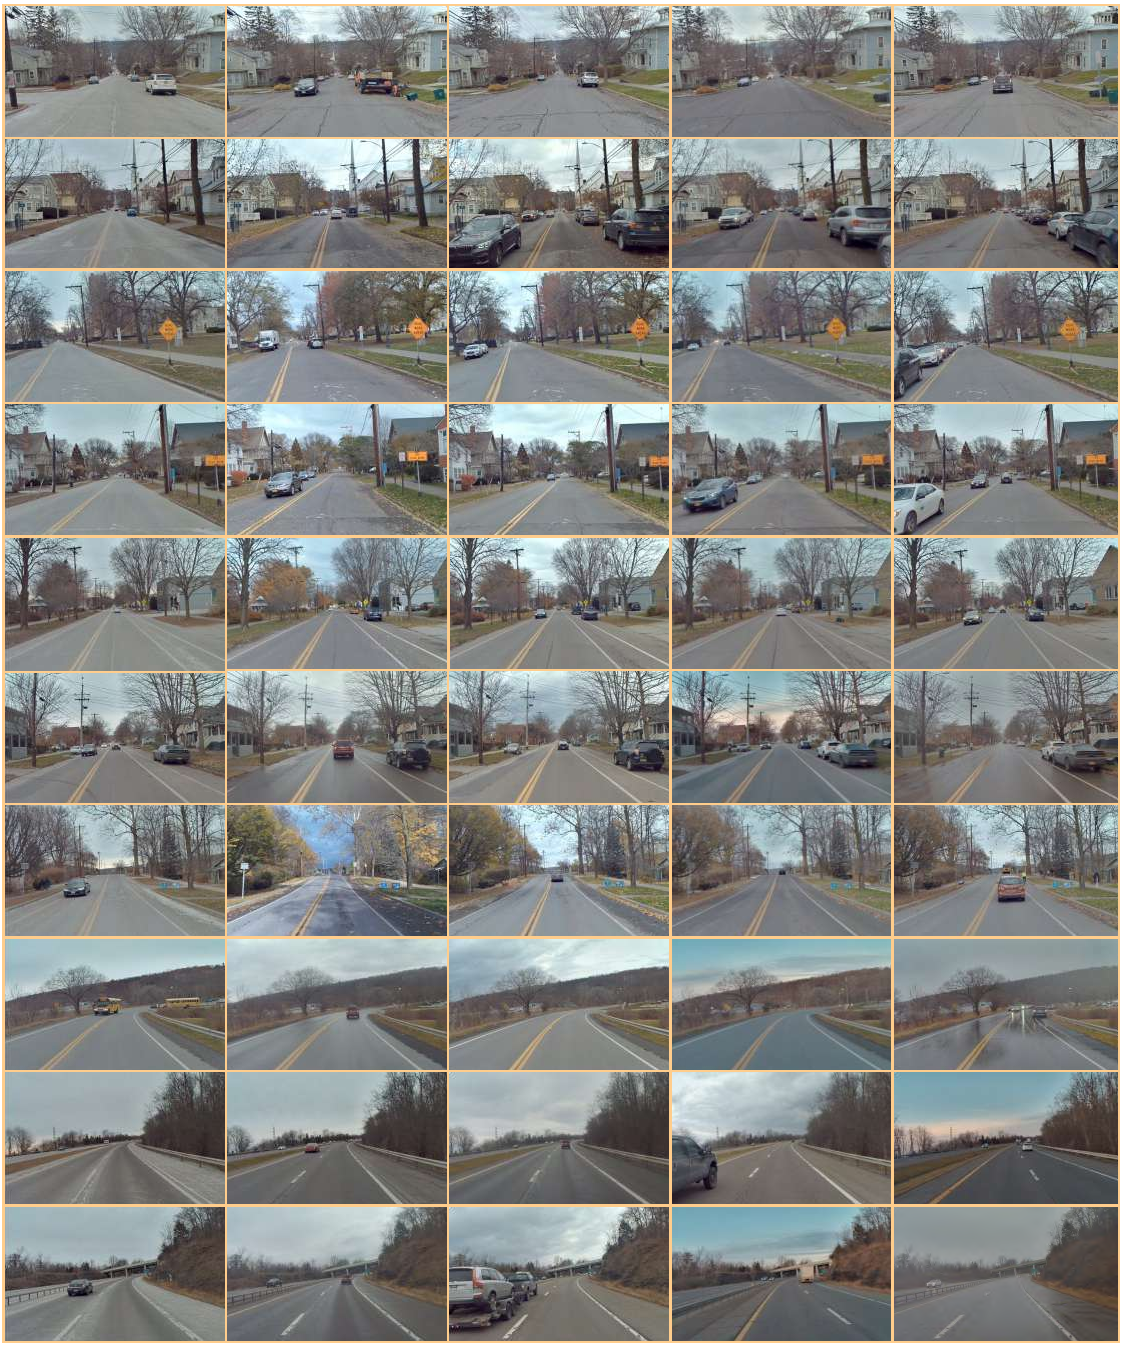
\includegraphics[width=0.95\linewidth]{figs_compressed/ithaca-1_compressed.pdf}
    \caption{\textbf{Visualizations of Mapverse-Ithaca365 dataset (locations 1-10).} Each row represents image observations of the same location captured during different traversals, with five traversals shown for brevity. The figure encompasses diverse environments in the Ithaca area, from residential neighborhoods with houses, trees, and varying traffic, to suburban streets with signage and seasonal foliage changes, and finally to rural roads and highways with expansive landscapes. The columns provide comparative views of these locations under different conditions, highlighting the dynamic nature of the Mapverse-Ithaca365 dataset.}
    \label{fig:ithaca-1}
\end{figure}

\begin{figure}
    \centering
    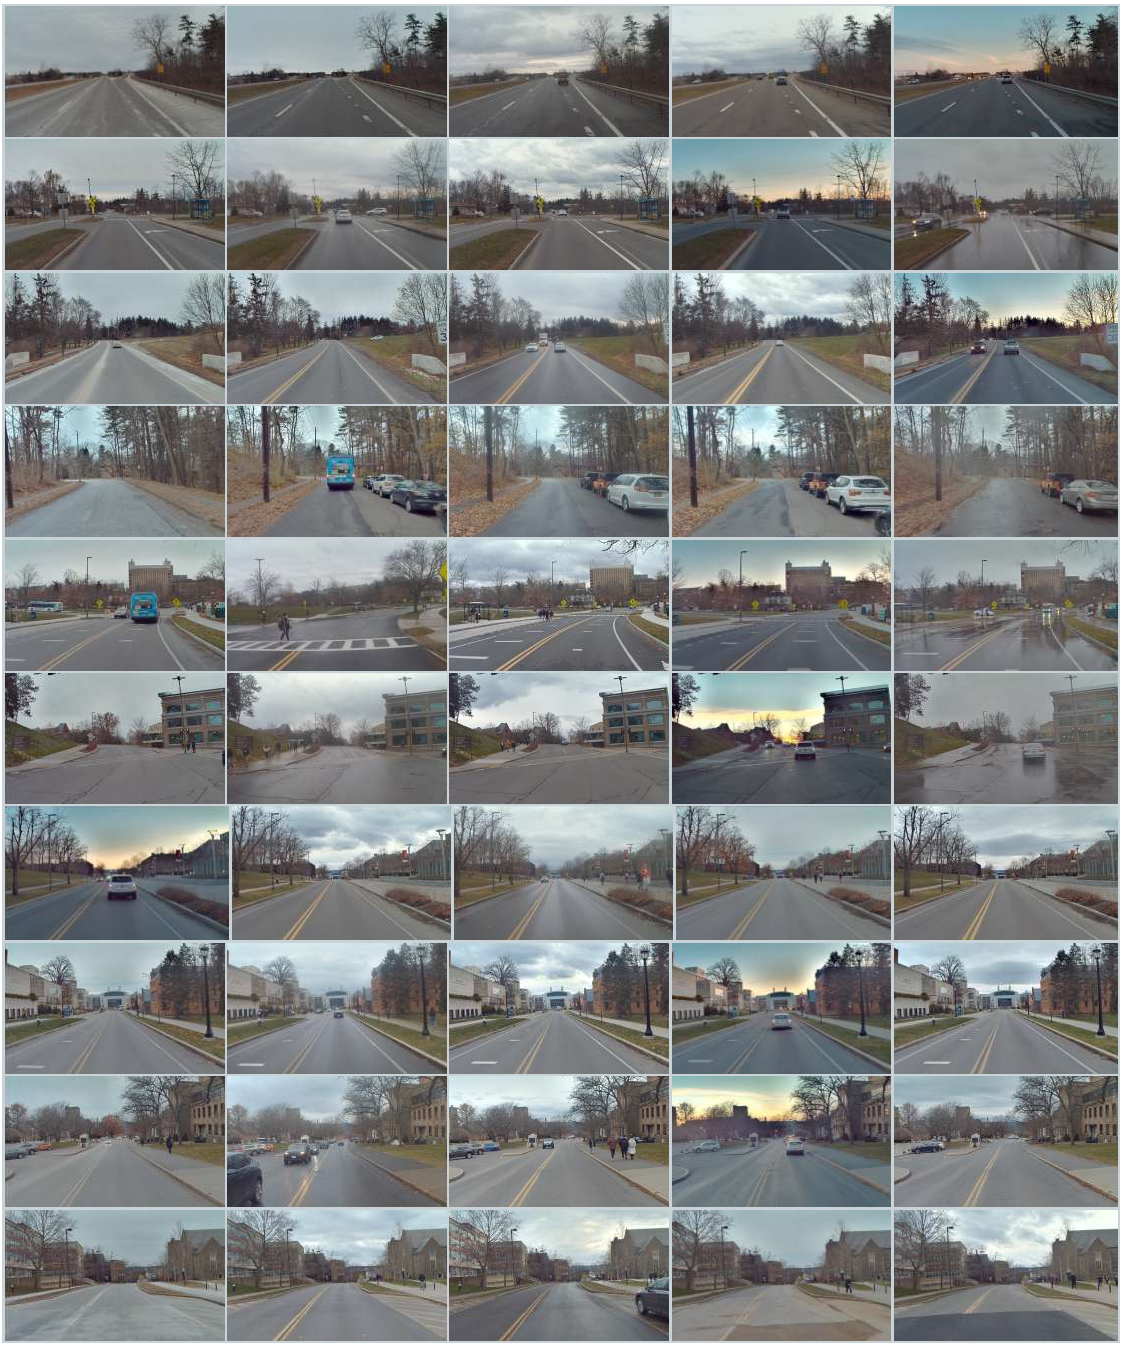
\includegraphics[width=1\linewidth]{figs_compressed/ithaca-2_compressed.pdf}
    \caption{\textbf{Visualizations of Mapverse-Ithaca365 dataset (locations 11-20).} Each row captures image observations of the same location from different traversals, showing five traversals for brevity. The figure spans various environments within Ithaca, from expansive rural highways transitioning to suburban roads with clear signage, to wooded areas with parked vehicles, and urban intersections with notable buildings. The images depict the progression from rural outskirts to more densely populated urban centers, reflecting changes in traffic, lighting, and seasonal foliage. Columns provide comparative views of these locations under different conditions, emphasizing the dynamic and diverse nature of the Mapverse-Ithaca365 dataset.}
    \label{fig:ithaca-2}
\end{figure}

\begin{figure}
    \centering
    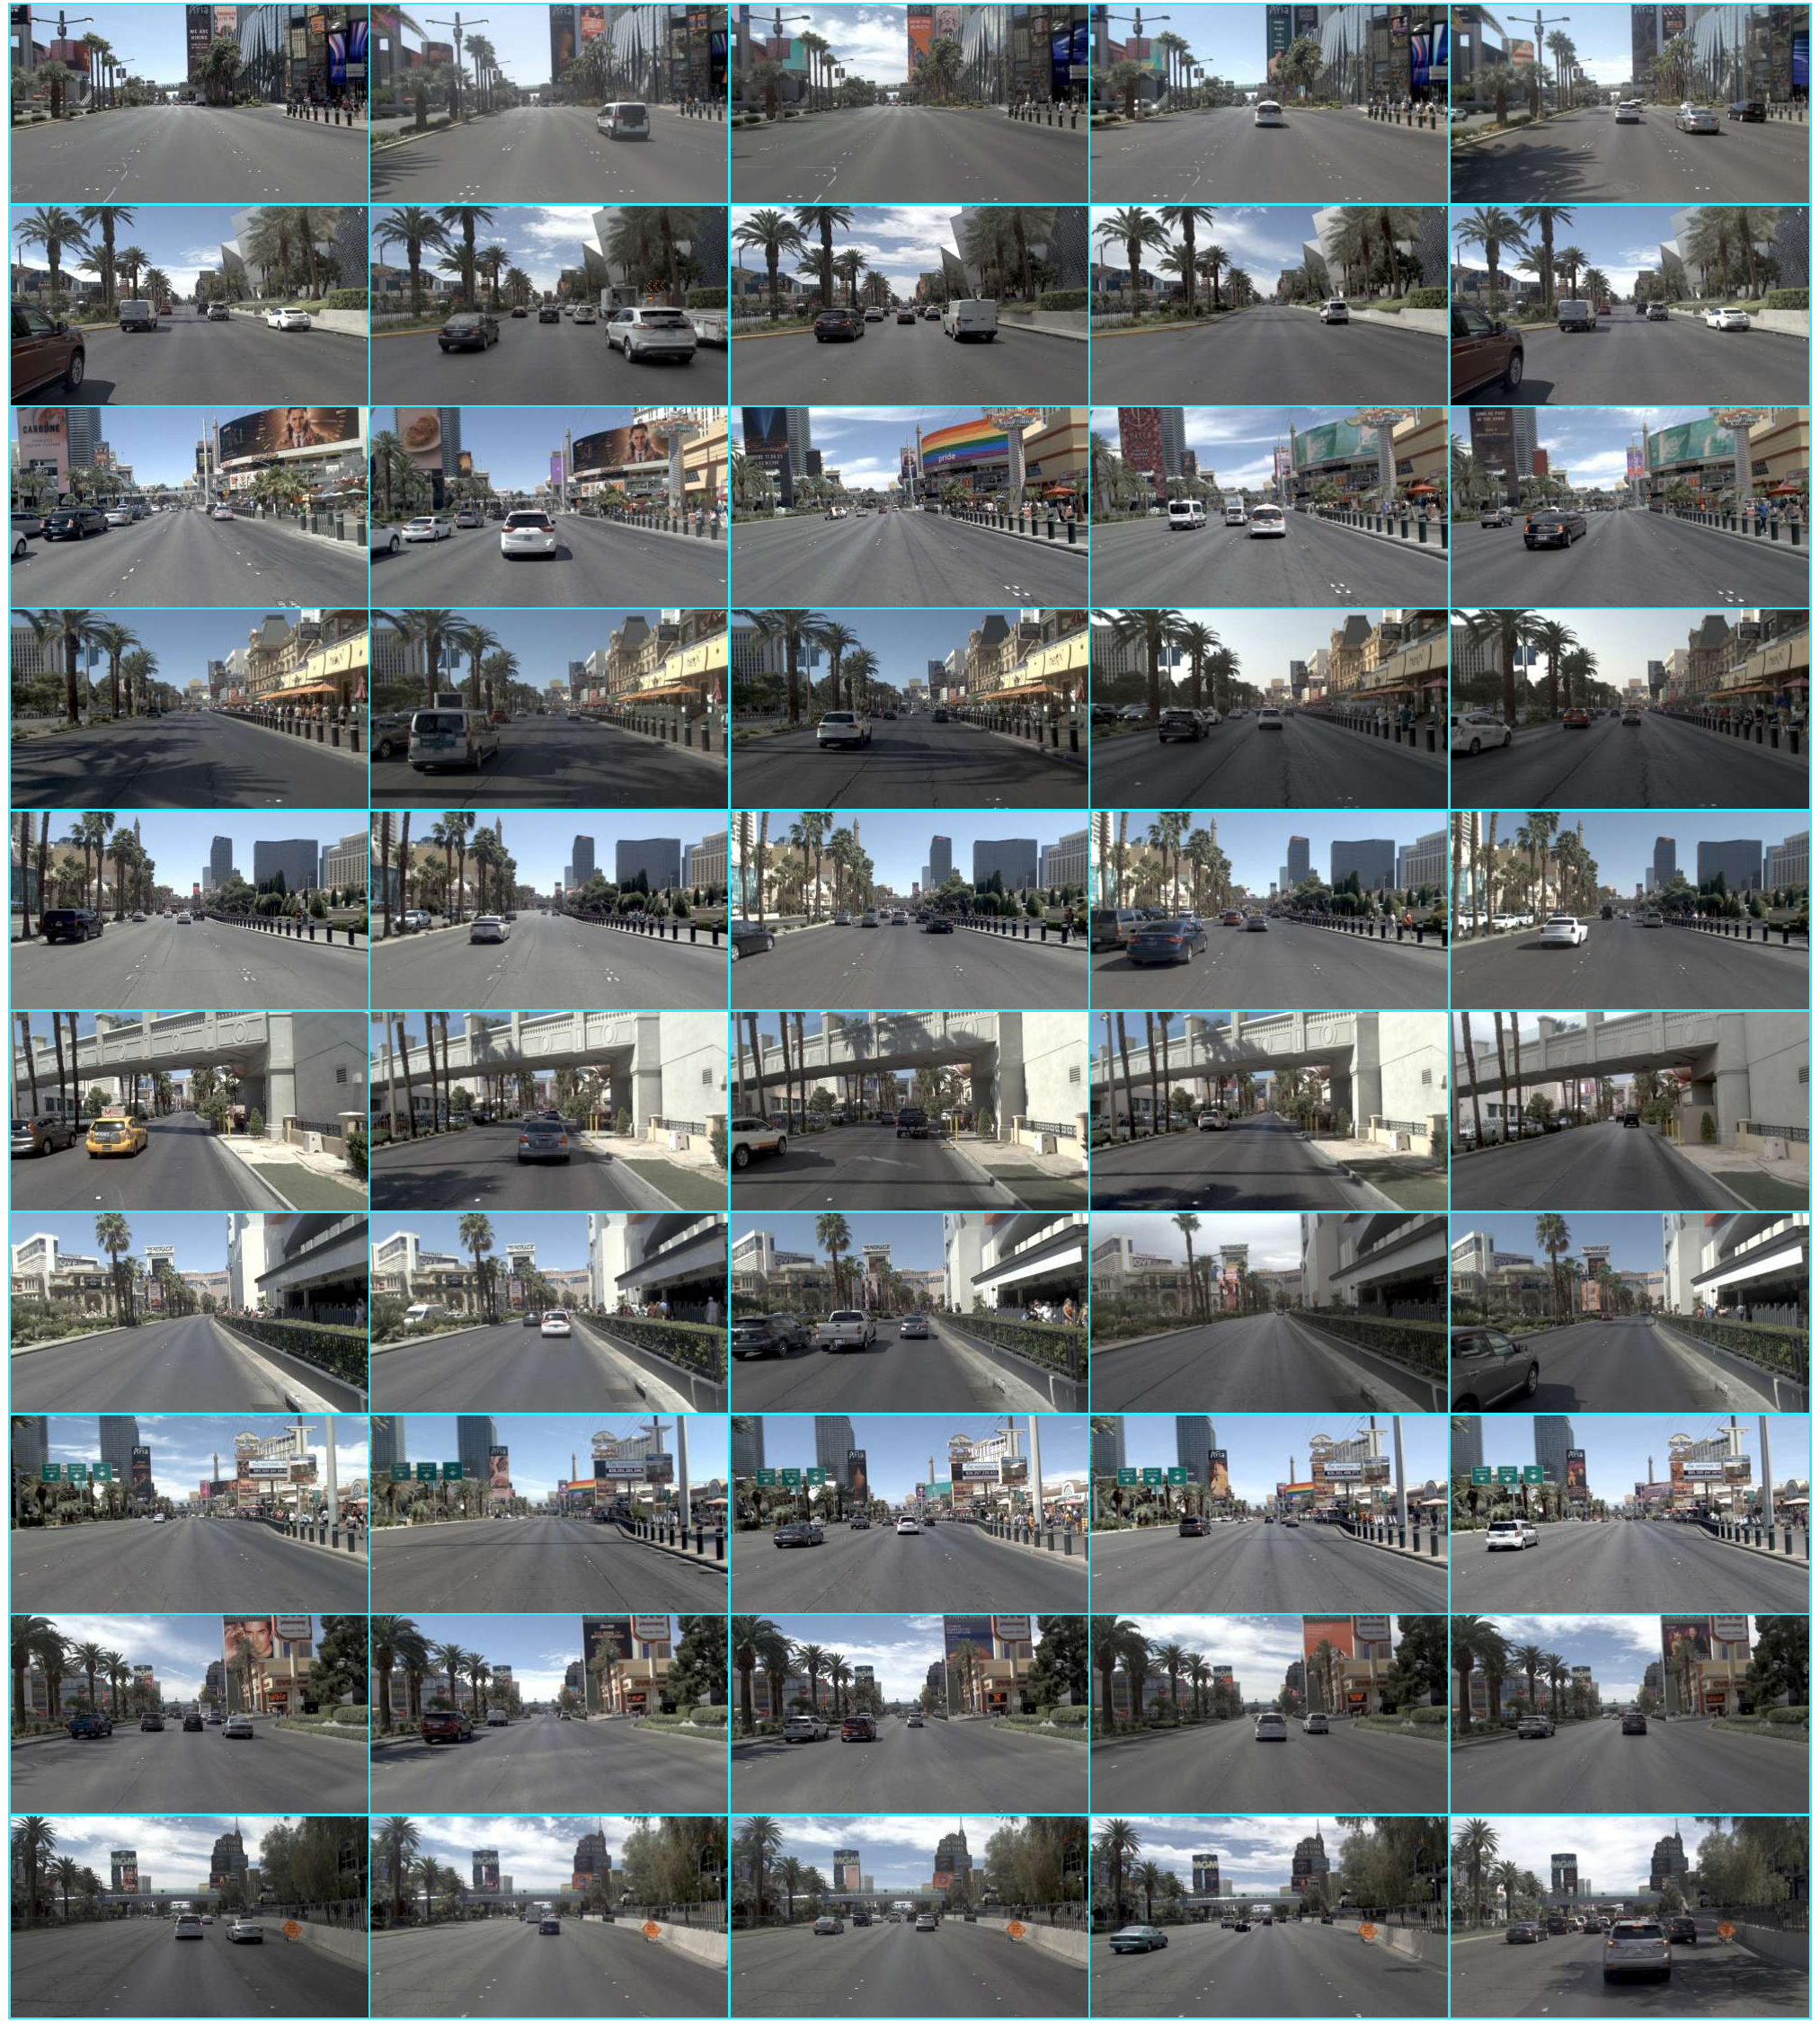
\includegraphics[width=1\linewidth]{figs_compressed/vegas-1_compressed.pdf}
    \caption{\textbf{Visualizations of Mapverse-nuPlan dataset (locations 1-10).} Each row represents different image observations of the same location captured during multiple traversals, with five shown for brevity. The images encompass diverse environments in Las Vegas, including wide city streets with iconic buildings, billboards, palm trees, pedestrian bridges, and varying traffic conditions.  Columns provide comparative views of the same locations under different conditions, illustrating the variability and complexity of the cityscape as captured in the Mapverse-nuPlan dataset.
}
    \label{fig:nuplan-1}
\end{figure}

\begin{figure}
    \centering
    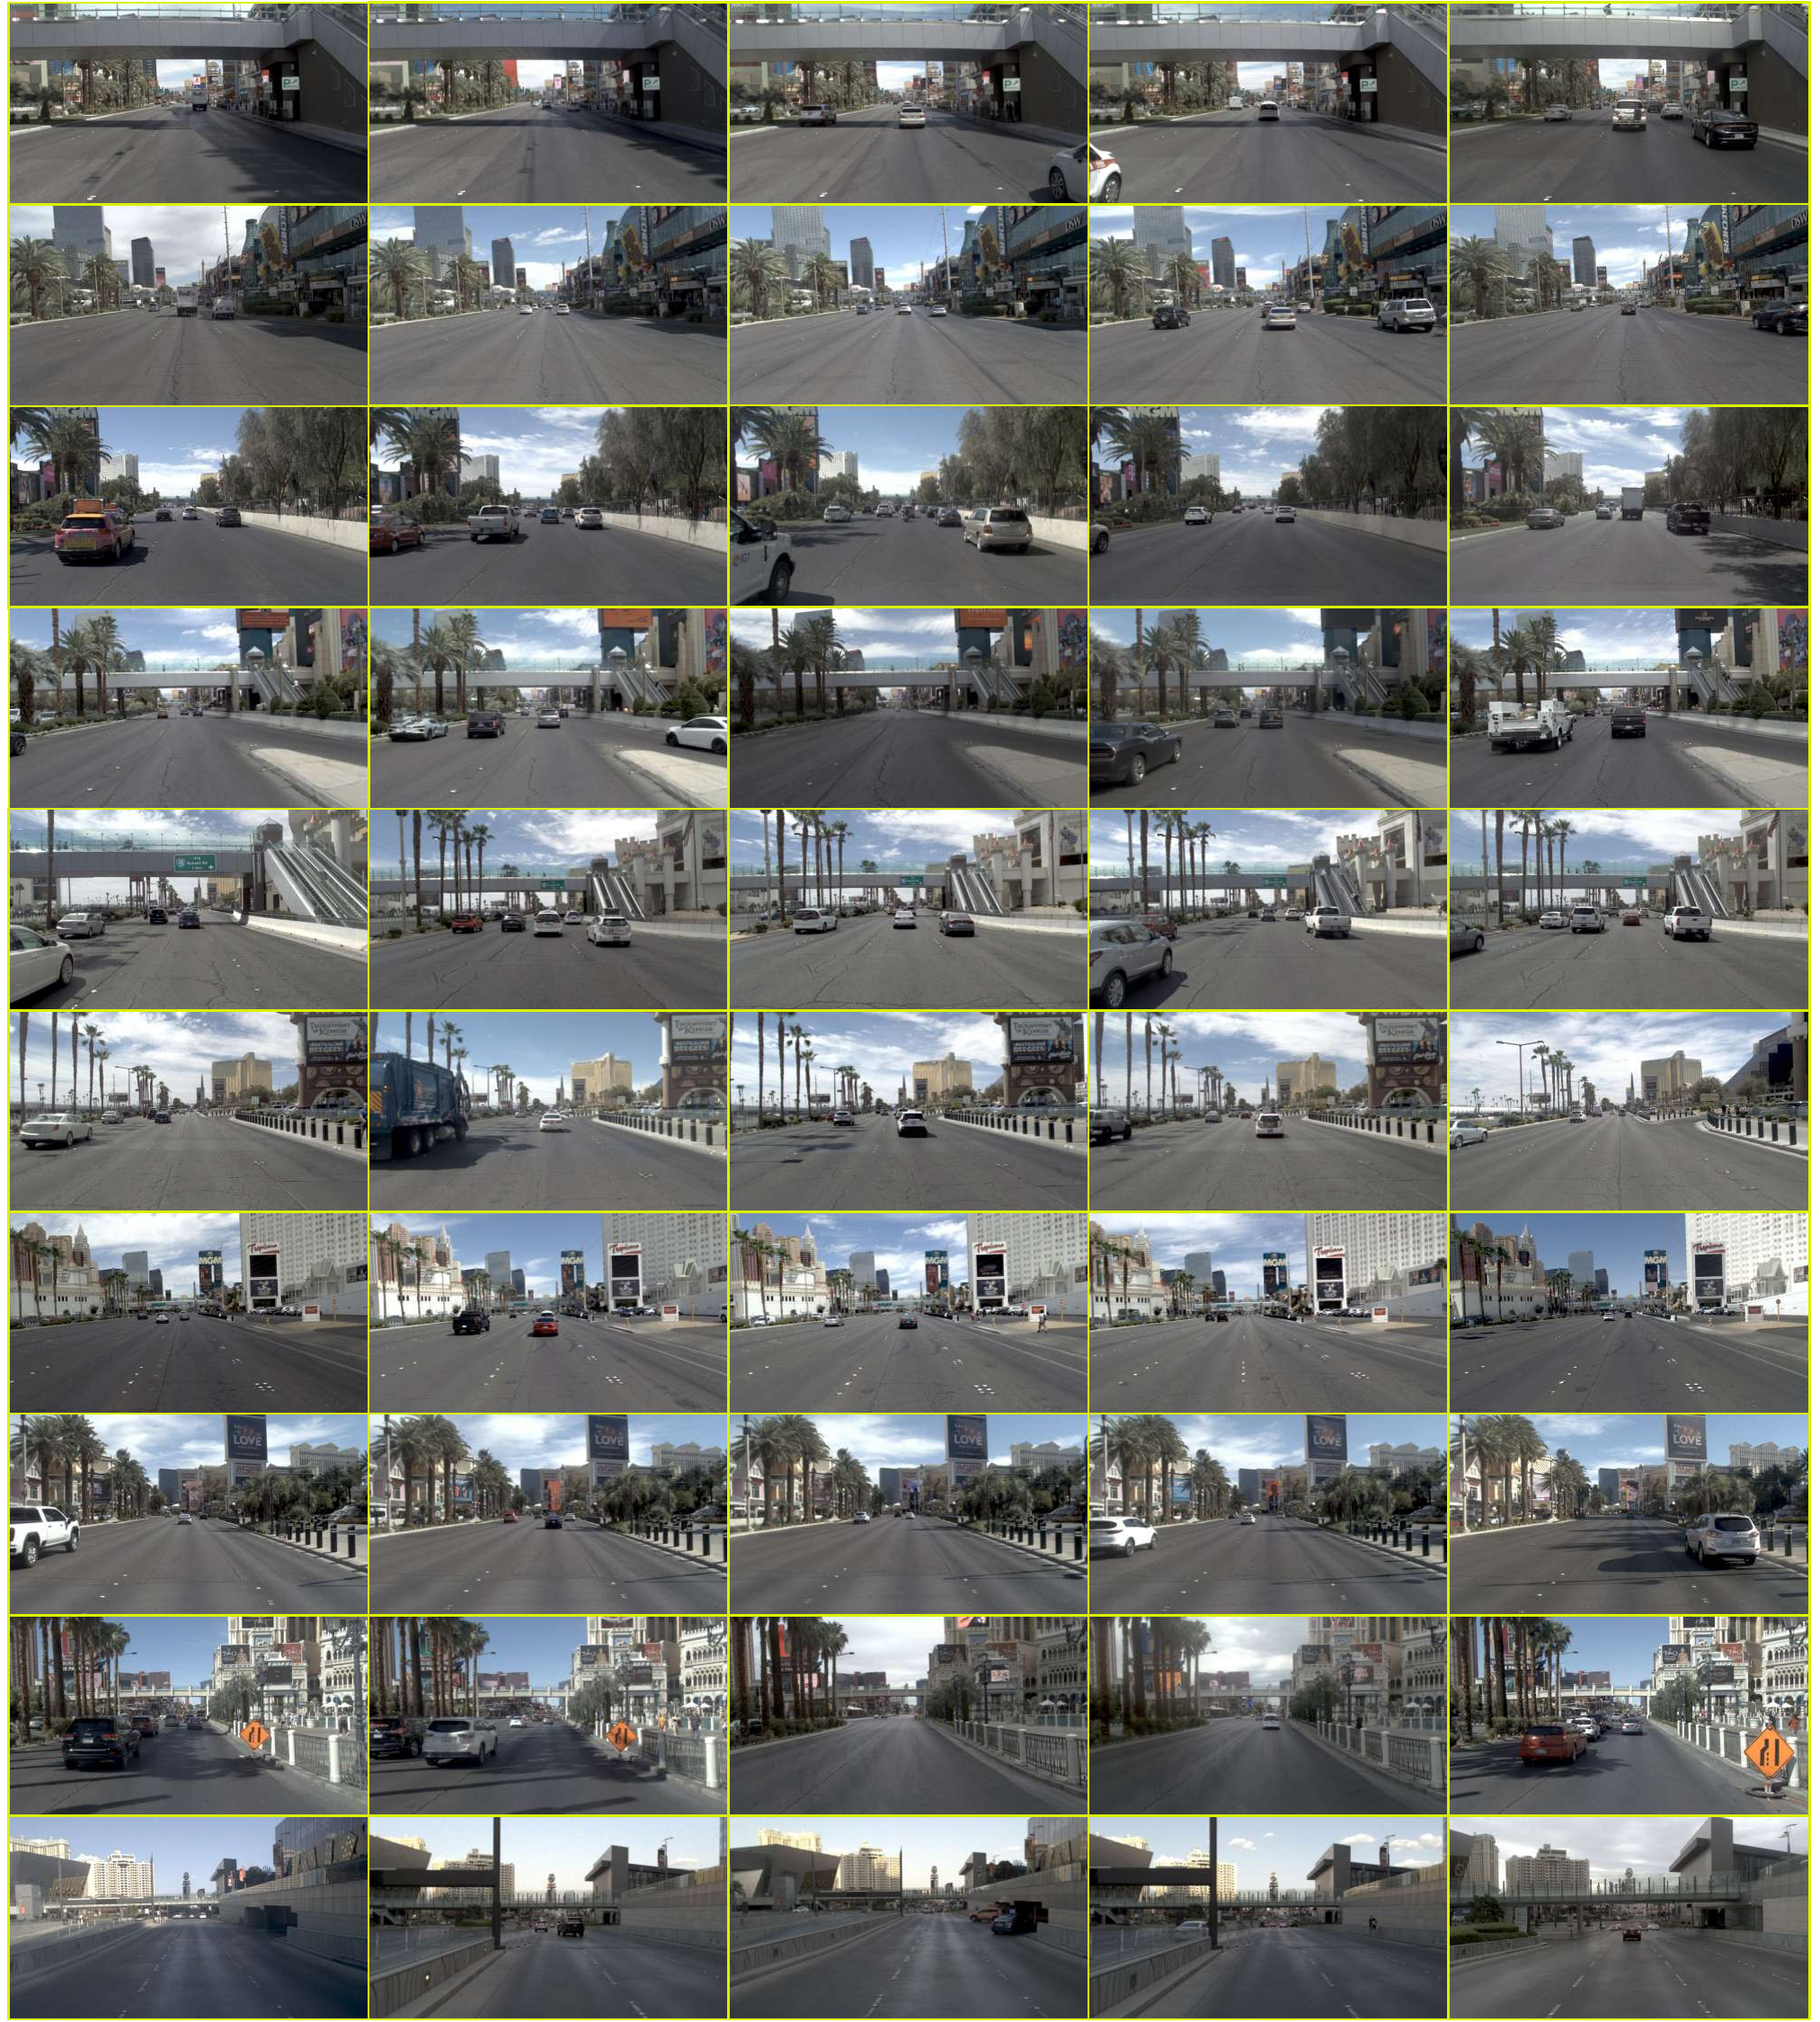
\includegraphics[width=1\linewidth]{figs_compressed/vegas-2_compressed.pdf}
    \caption{\textbf{Visualizations of Mapverse-nuPlan dataset (locations 11-20).} Each row represents different image observations of the same location captured during multiple traversals, with five shown for brevity. The images cover various environments in Las Vegas, including city streets with overpasses, iconic buildings, palm trees, billboards, and varied traffic conditions. The sequence progresses from urban settings with heavy infrastructure and prominent landmarks to broader streets and intersections, capturing different times of day and lighting conditions. Columns provide comparative views of the same locations under different circumstances, showcasing the dynamic and ever-changing urban landscape of Las Vegas as recorded in the Mapverse-nuPlan dataset.}
    \label{fig:nuplan-2}
\end{figure}


\clearpage


\section{Mapverse-Ithaca365: Additional Results of 2D Segmentation}
\subsection{Additional Qualitative Results}
\label{subsec:add-quali-appendix}
\begin{figure}[ht]
\begin{center}
\centerline{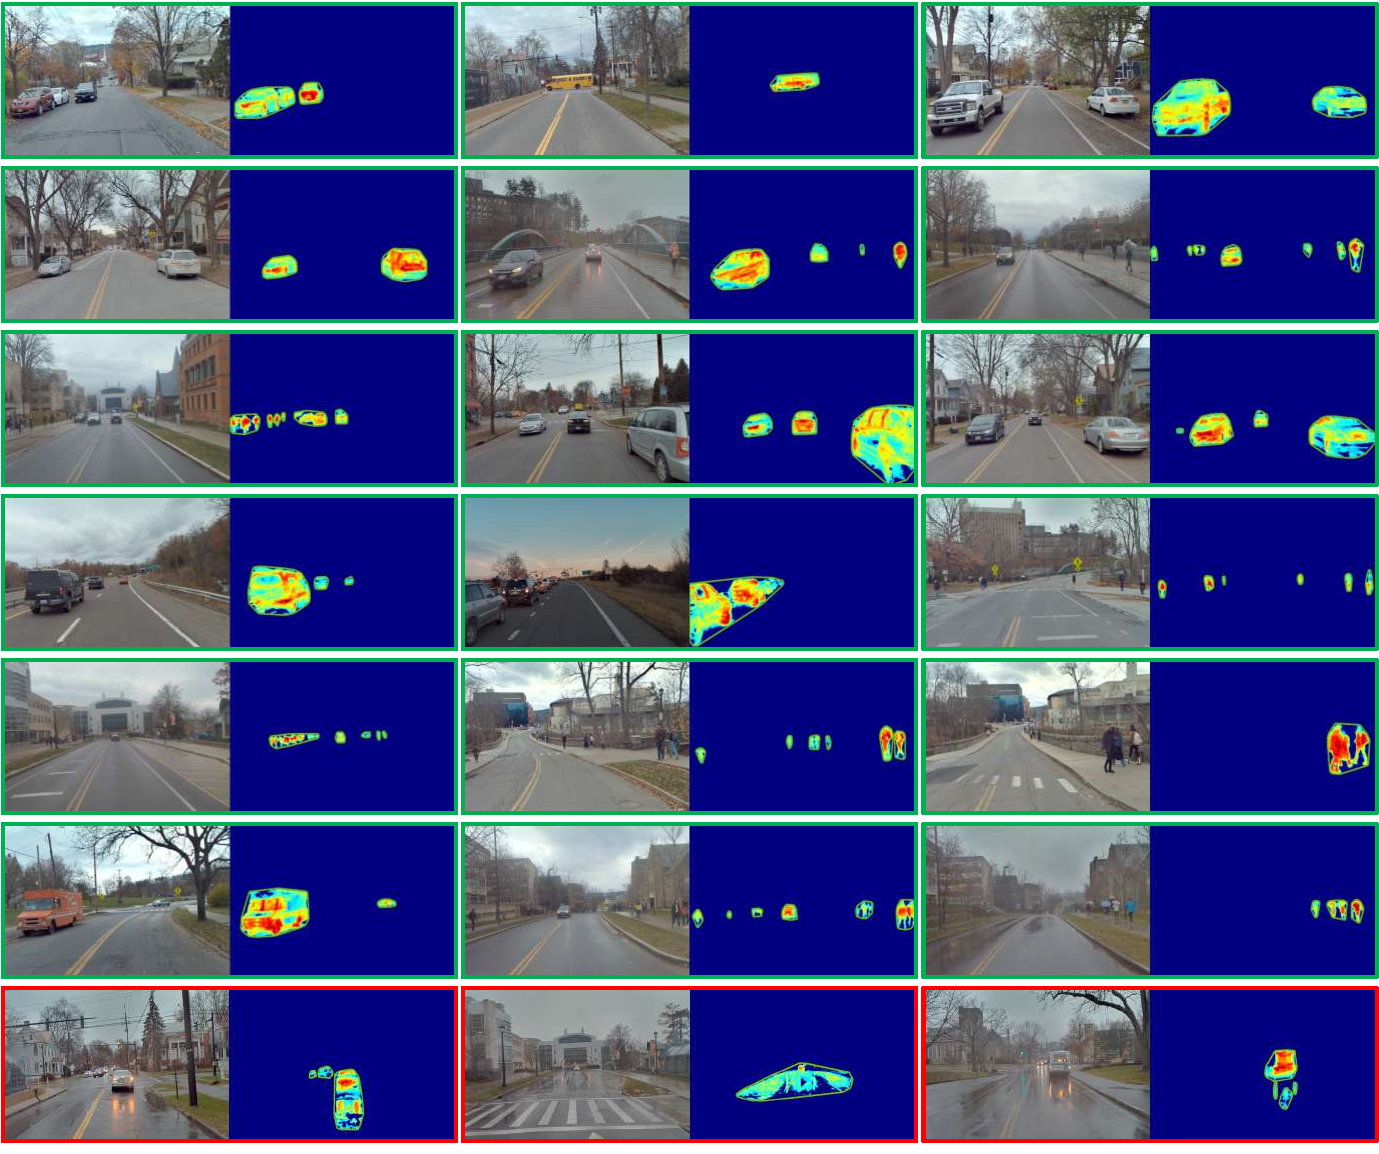
\includegraphics[width=\columnwidth]{figs_compressed/featmask-supp_compressed.pdf}}
\caption{\textbf{Qualitative evaluations of the emerged object masks}. Our method demonstrates robust performance across a range of lighting and weather conditions, effectively handling diverse categories including cars, buses, and pedestrians. Some failure cases are highlighted with red rectangles. }
\label{fig:visseg-appendix}
\end{center}
% \vspace{-10mm}
\end{figure}


\clearpage

\subsection{Visualizations of Supervised and Unsupervised Segmentation}


\label{subsec:vis-compareison-appendix}
\begin{figure}[ht]
\begin{center}
\centerline{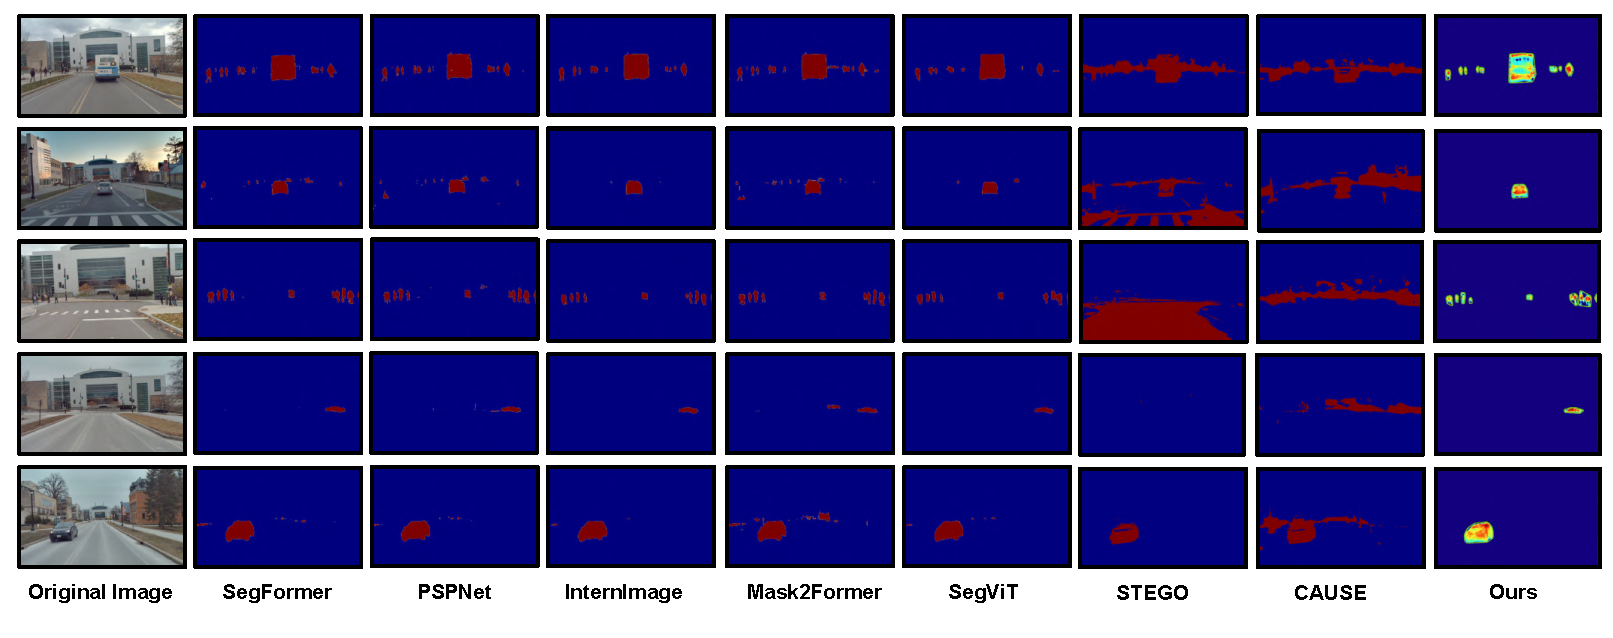
\includegraphics[width=\columnwidth]{figs_compressed/seg-compare_compressed.pdf}}
\caption{\textbf{Qualitative comparisons of our method and other supervised and unsupervised segmentation baselines.} This image demonstrates a comparison between our mask extraction and those derived from other semantic segmentation methods. The results indicate that our masks maintain superior integrity and detail in complex environments. Meanwhile, our method significantly outperforms unsupervised semantic segmentation models~\cite{hamilton2022unsupervised,kim2023causal} and is roughly equivalent to the masks generated by InternImage~\cite{wang2023internimage} and SegVit~\cite{zhang2022segvit}. Although Mask2Former~\cite{cheng2022masked}, PSPNet~\cite{zhao2017pspnet}, and SegFormer~\cite{xie2021segformer} have advantages in recognizing people and other fine-grained objects, they can also lead to incorrect segmentation and noise in certain scenarios. }
\label{fig:comparison-seg-appendix}
\end{center}
\vspace{-10mm}
\end{figure}

\clearpage

\subsection{Performance over Training Iterations }

Figure~\ref{fig:ablation-iteration-appendix} presents the IoU performance across iterations for two different feature resolutions (110×180 and 140×210), alongside visualizations of ephemerality masks and feature residuals at various iterations. The IoU graph on the left shows that both resolutions exhibit rapid improvement in the initial iterations, with the 110×180 resolution consistently outperforming the 140×210 resolution. The 110×180 resolution reaches an IoU of approximately 0.44, while the 140×210 resolution plateaus around 0.41. This indicates that the lower resolution (110×180) is more efficient in capturing ephemeral objects. On the right, the visualizations of ephemerality masks and feature residuals at different iterations (500 to 10000) demonstrate that higher iterations result in more detailed and accurate segmentation. Early iterations (500 and 1000) show sparse and less accurate masks. The progression also highlights the fast convergence of our method for effective segmentation.

\paragraph{Summary} In summary, the figure demonstrates that the 110×180 feature resolution is more effective and efficient for segmentation, achieving higher IoU scores compared to the 140×210 resolution. The IoU increases rapidly in the initial iterations and stabilizes around iteration 4000. These results emphasize the importance of selecting an appropriate feature resolution and ensuring sufficient iterations to achieve optimal segmentation performance.

\vspace{5mm}

\begin{figure}[ht]
\begin{center}
\centerline{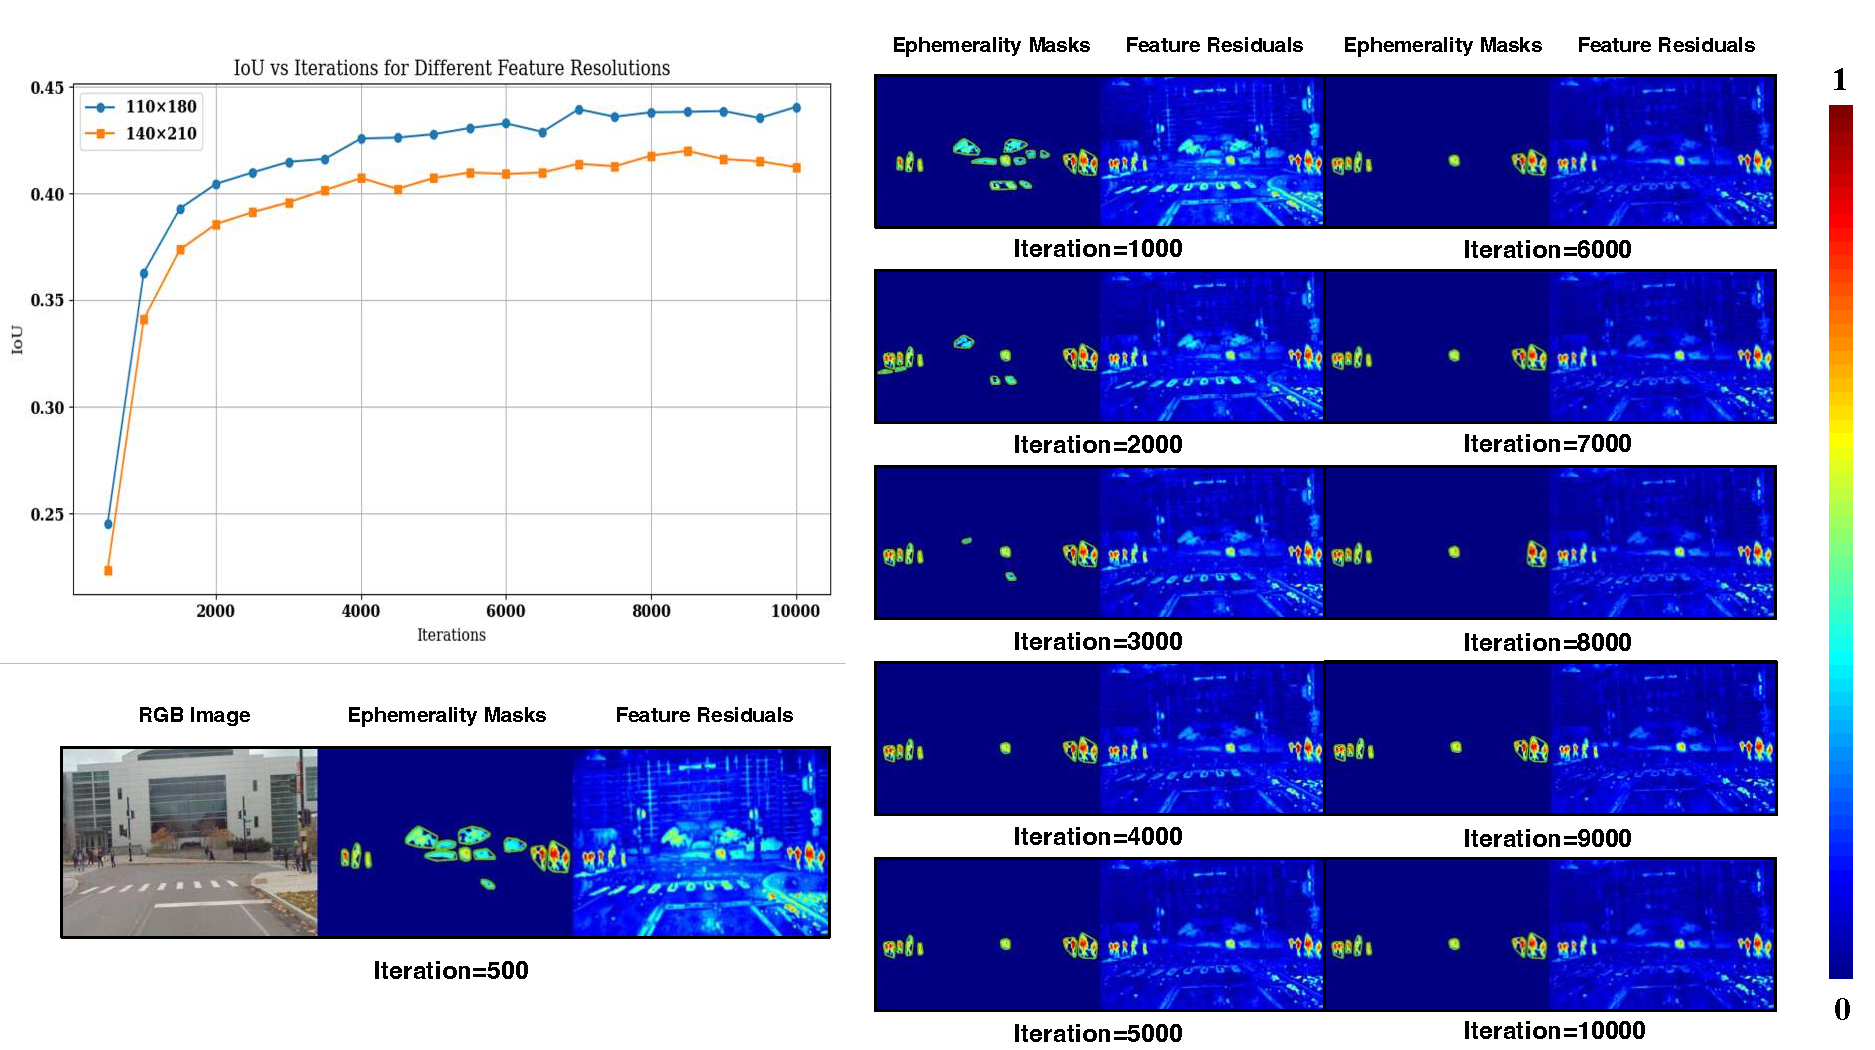
\includegraphics[width=\columnwidth]{figs_compressed/ablation-iteration_compressed.pdf}}
\caption{ \textbf{IoU performance over iterations for different feature resolutions (110×180 and 140×210) and corresponding visualizations of ephemerality masks and feature residuals.} Visualizations at various iterations (500 to 10000) illustrate that higher iterations lead to more detailed and accurate segmentation. The results highlight the efficiency of the 110×180 resolution and the fast convergence of our method for effective segmentation.}
\label{fig:ablation-iteration-appendix}
\end{center}
\end{figure}





\clearpage




\subsection{Ablation Study on Number of Traversal: Visualization and Discussion}

Figure~\ref{fig:ablation-traversal-appendix} showcases the segmentation performance of \texttt{EmerSeg} with images collected from varying numbers of traversals. Each row represents a different scene, while the columns illustrate the results from 1, 2, 3, 7, and 10 traversals, respectively. The segmentation map with a single traversal shows minimal detection of ephemeral objects, indicating limited information for effective segmentation. For example, the method fails to segment three parked buses in the first row due to a lack of diverse visual observations, which are crucial for our model to localize these transient yet static objects. With 2 traversals, there is a significant improvement in segmentation performance. The segmentation map reveals larger and more distinct objects, demonstrating the benefit of additional traversals. Segmentation performance with 10 traversals is similar to that with 7 traversals. Objects are detected reliably, but the improvement beyond 7 traversals is marginal, indicating diminishing returns.


\paragraph{Summary} Figure~\ref{fig:ablation-traversal-appendix} illustrates the clear trend of improving segmentation performance with an increasing number of traversals. The results indicate that while significant gains are achieved with additional traversals, the benefits plateau after a certain point. This analysis underscores the importance of multiple traversals for effective segmentation while suggesting an optimal balance between the number of traversals and segmentation accuracy.


\vspace{5mm}


\begin{figure}[ht]
\begin{center}
\centerline{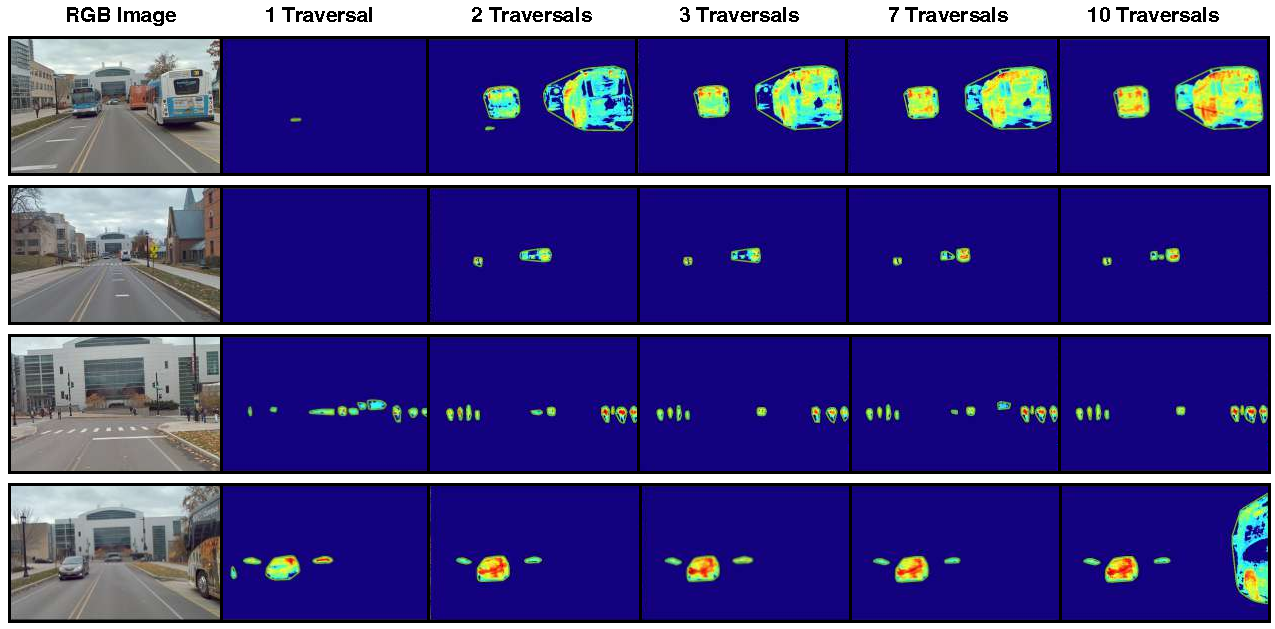
\includegraphics[width=\columnwidth]{figs_compressed/ablation-traversal_compressed.pdf}}
\caption{\textbf{Visualizations of \texttt{EmerSeg} with inputs from different numbers of traversals.} Each row represents a different scene of a location. The first column shows the original RGB images. The subsequent columns show the segmentation outputs from \texttt{EmerSeg} with 1, 2, 3, 7, and 10 traversals.}
\label{fig:ablation-traversal-appendix}
\end{center}
\end{figure}

\clearpage





\subsection{Ablation Study on Feature Dimension: Visualization and Discussion}

Figure~\ref{fig:ablation-dimension-appendix} illustrates the impact of varying feature dimensions on the segmentation performance. At the lowest dimension (4), the ephemerality masks are sparse, capturing very few objects with minimal detail since the feature residuals are not discriminative, indicating insufficient feature representation. A substantial enhancement is observed at dimension 16, where the ephemerality masks become more detailed, capturing more objects with better clarity. At the highest dimension (64), the segmentation is highly detailed and accurate, with ephemerality masks capturing a wide range of objects and feature residuals being informative, suggesting a comprehensive feature representation.

\paragraph{Summary} In summary, the segmentation performance improves significantly with increased feature dimensions. Low-dimensional features (4 and 8) fail to provide adequate information for accurate segmentation, resulting in sparse segmentation. A higher dimension (16 and 64) offers a substantial improvement, capturing most objects with clearer details. This demonstrates that higher-dimensional features are crucial for achieving accurate and comprehensive segmentation performance.

\vspace{5mm}

\begin{figure}[ht]
\begin{center}
\centerline{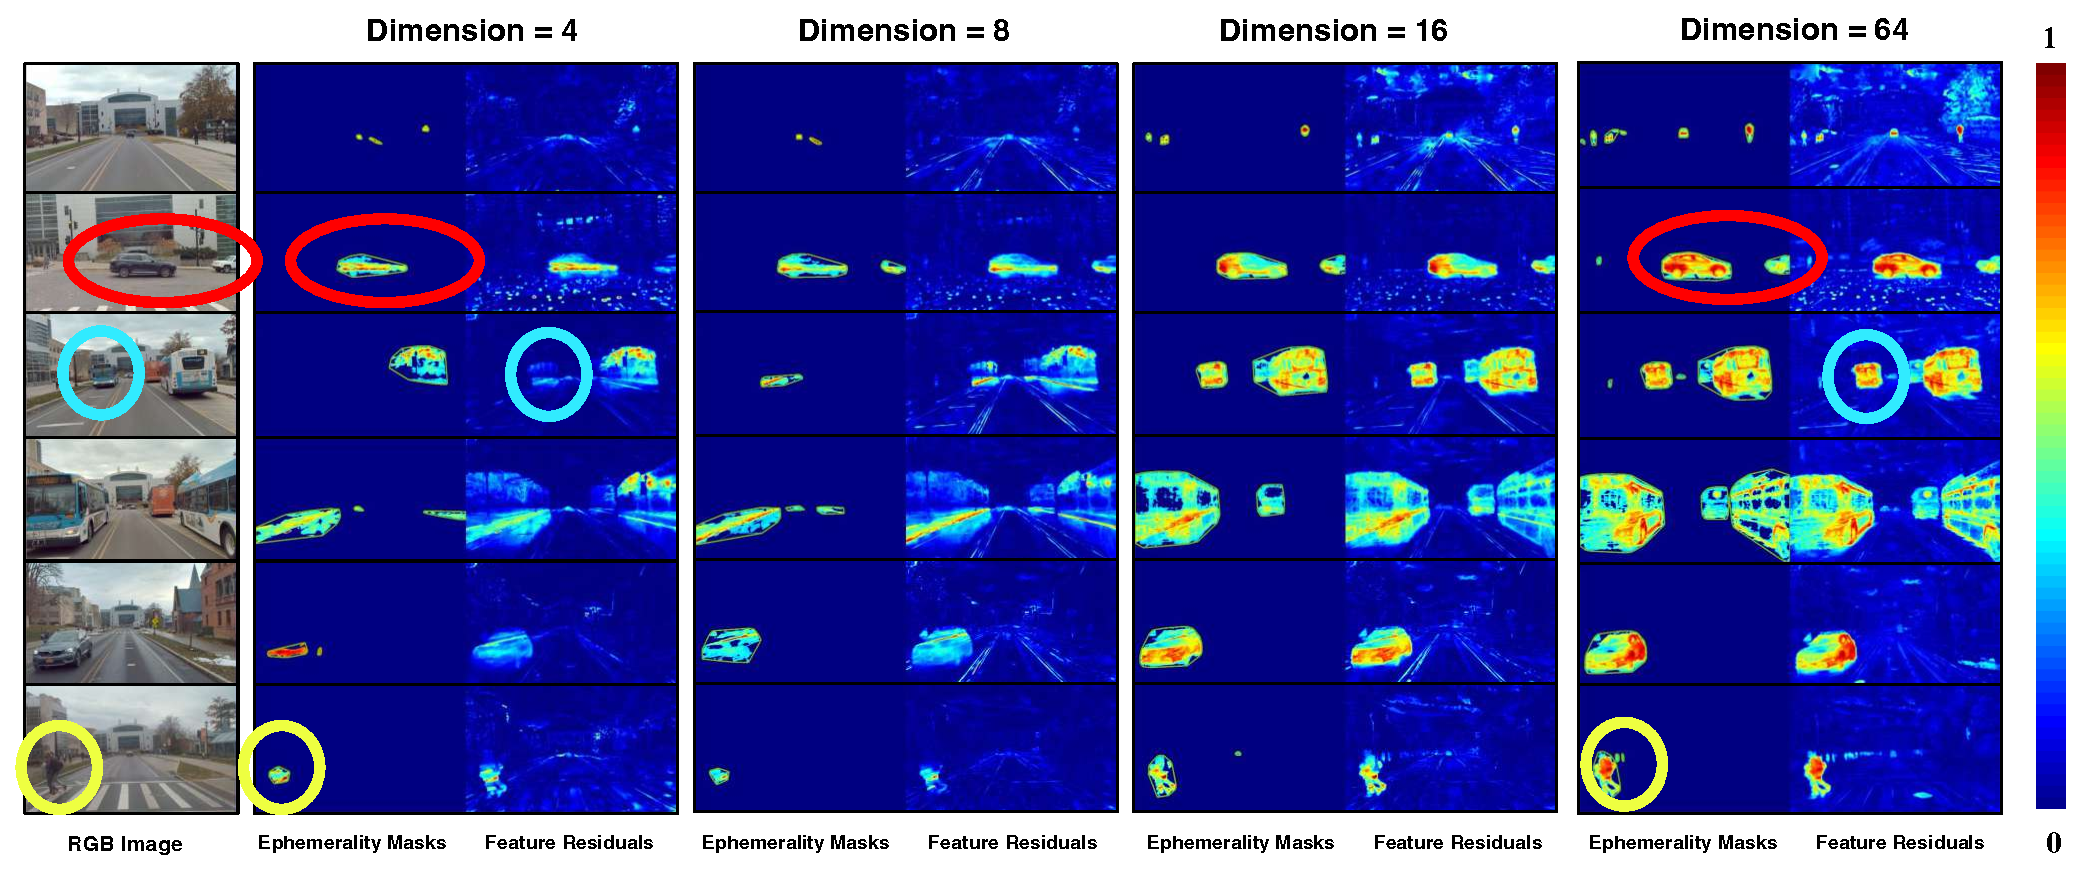
\includegraphics[width=\columnwidth]{figs_compressed/ablation-dimension_compressed.pdf}}
\caption{\textbf{Visualizations of ephemerality masks and feature residuals at different feature dimensions.} The RGB images (leftmost column) are processed to generate ephemerality masks and feature residuals. As the feature dimensions increase, the segmentation accuracy improves, with the highest dimension (64) capturing the most detailed and accurate object masks. The residuals are more discriminative with higher dimensions, indicating better feature representation. The colored circles highlight specific areas to illustrate differences in segmentation quality across dimensions.}
\label{fig:ablation-dimension-appendix}
\end{center}
\end{figure}

\clearpage




\subsection{Ablation Study on Feature Resolution: Visualization and Discussion}

Figure~\ref{fig:ablation-resolution-appendix} presents the segmentation performance at different feature resolutions: 25×40, 50×80, 70×110, and 110×180. The RGB images on the left are segmented into ephemerality masks and feature residuals for each resolution. At the lowest resolution (25×40), the ephemerality masks capture very few objects with minimal detail. As the resolution increases, there is a noticeable improvement in object segmentation, with more objects being identified. 

\paragraph{Summary} In a word, the segmentation performance improves significantly with increased feature resolution. Lower resolutions (25×40 and 50×80) result in sparse object segmentation, indicating inadequate feature representation. The highest resolution (110×180) delivers the best results, with detailed and precise segmentation. 

\vspace{5mm}
\begin{figure}[ht]
\begin{center}
\centerline{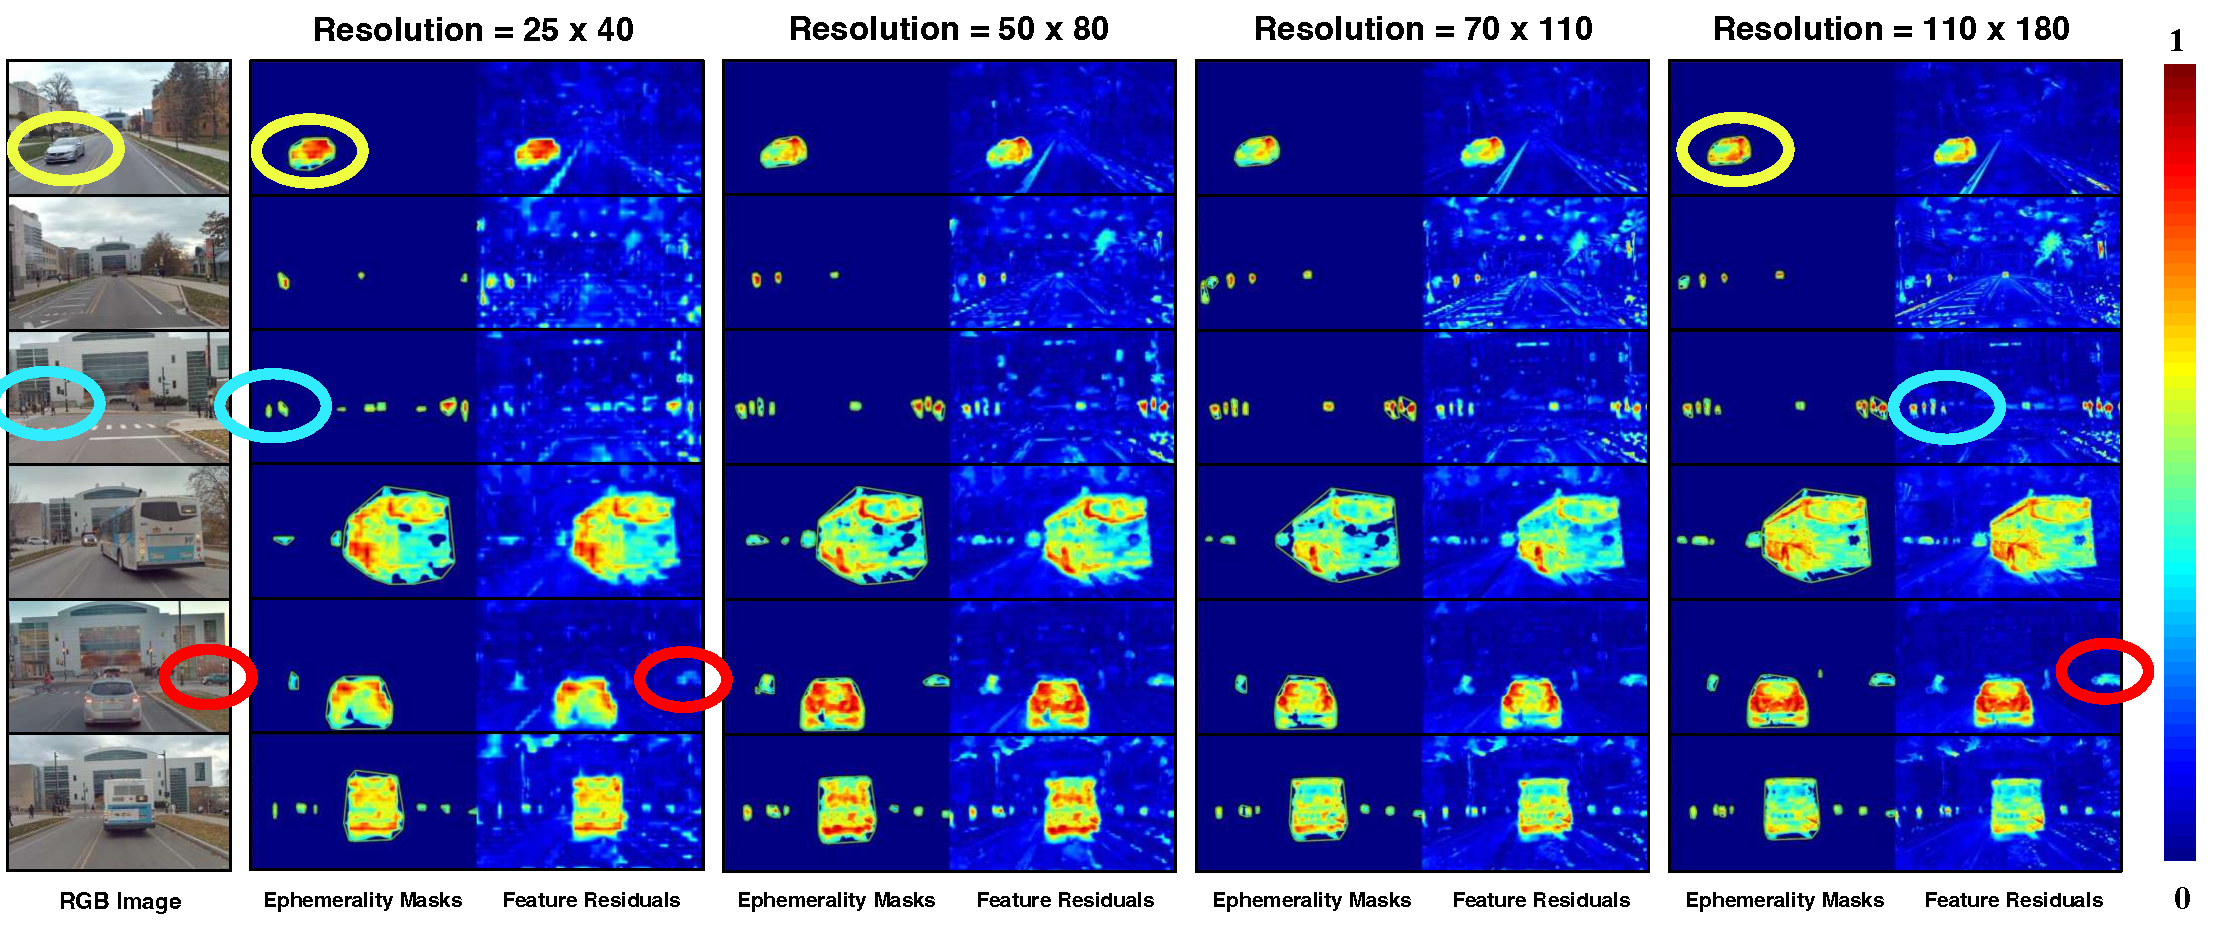
\includegraphics[width=\columnwidth]{figs_compressed/ablation-resolution_compressed.pdf}}
\caption{\textbf{Visualizations of ephemerality masks and feature residuals at different feature (spatial) resolutions.} The RGB images (leftmost column) are processed to generate ephemerality masks and feature residuals. As the feature resolution increases, the segmentation accuracy improves, with the highest resolution (110×180) capturing the most detailed and accurate object masks. The residuals are more informative with higher resolutions, indicating better feature representation and reduced segmentation errors. The colored circles highlight specific areas to illustrate differences in segmentation quality across resolutions.}
\label{fig:ablation-resolution-appendix}
\end{center}
\end{figure}



\clearpage






\subsection{Ablation Study on Vision Foundation Model: Visualization and Discussion}

Figure~\ref{fig:ablation-backbone-appendix} compares the performance of different versions and configurations of the DINO model on ephemerality masks and feature residuals. For both DINOv1 and DINOv2, the raw versions show noisy feature residuals, indicating areas where the model fails to capture ephemeral objects accurately. The denoised versions show a notable improvement, with informative residuals and more accurate ephemerality masks. The DINOv2 models generally perform better than DINOv1, as evidenced by more precise object masks and more discriminative residuals. The inclusion of the register in DINOv2 does not introduce additional gains.

\paragraph{Summary} The result highlights the progressive improvements in segmentation accuracy achieved through model evolution from DINOv1 to DINOv2, and the benefits of applying denoising techniques. 

\vspace{5mm}
\begin{figure}[ht]
\begin{center}
\centerline{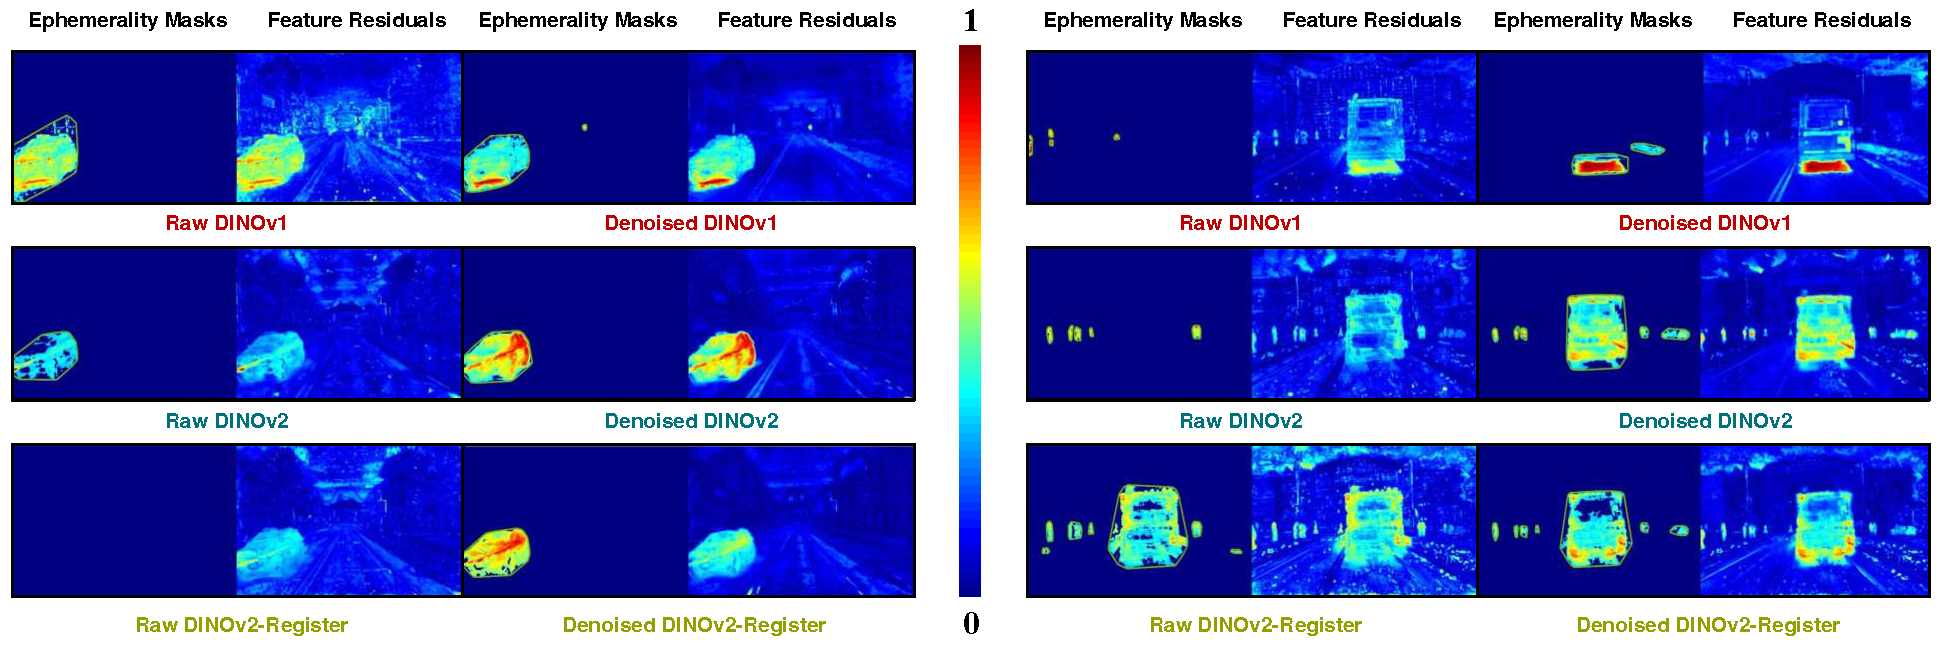
\includegraphics[width=\columnwidth]{figs_compressed/ablation-backbone_compressed.pdf}}
\caption{\textbf{Comparison of ephemerality masks and feature residuals using different versions of the DINO model.} The figure includes raw and denoised versions of DINOv1 and DINOv2, as well as raw and denoised versions of DINOv2 with a registration module (DINOv2-Register). Denoising enhances the quality of feature residuals, while registration does not yield notable gains.}
\label{fig:ablation-backbone-appendix}
\end{center}
\end{figure}



\clearpage



\section{Mapverse-Ithaca365: Additional Visualizations of 3D Reconstruction}
Figure~\ref{fig:reconstruction-appendix} compares Structure from Motion (SfM) initialized points with Gaussian points after optimization. On the left, the images display the raw data points obtained from the SfM process, which serves as an initial guess for the 3D structure of the environment. These points tend to be more scattered and less organized. On the right, the images show the Gaussian points after optimization, where the point cloud data has been refined through differentiable rendering. This refinement results in a more coherent and precise representation of the scene, as evidenced by the clearer and more defined structures in the point clouds. The comparison across various scenes highlights the effectiveness of the optimization process in enhancing the accuracy and clarity of the 3D reconstructed environment, crucial for applications in autonomous driving and robotics. 

\begin{figure}[ht]
    \centering
    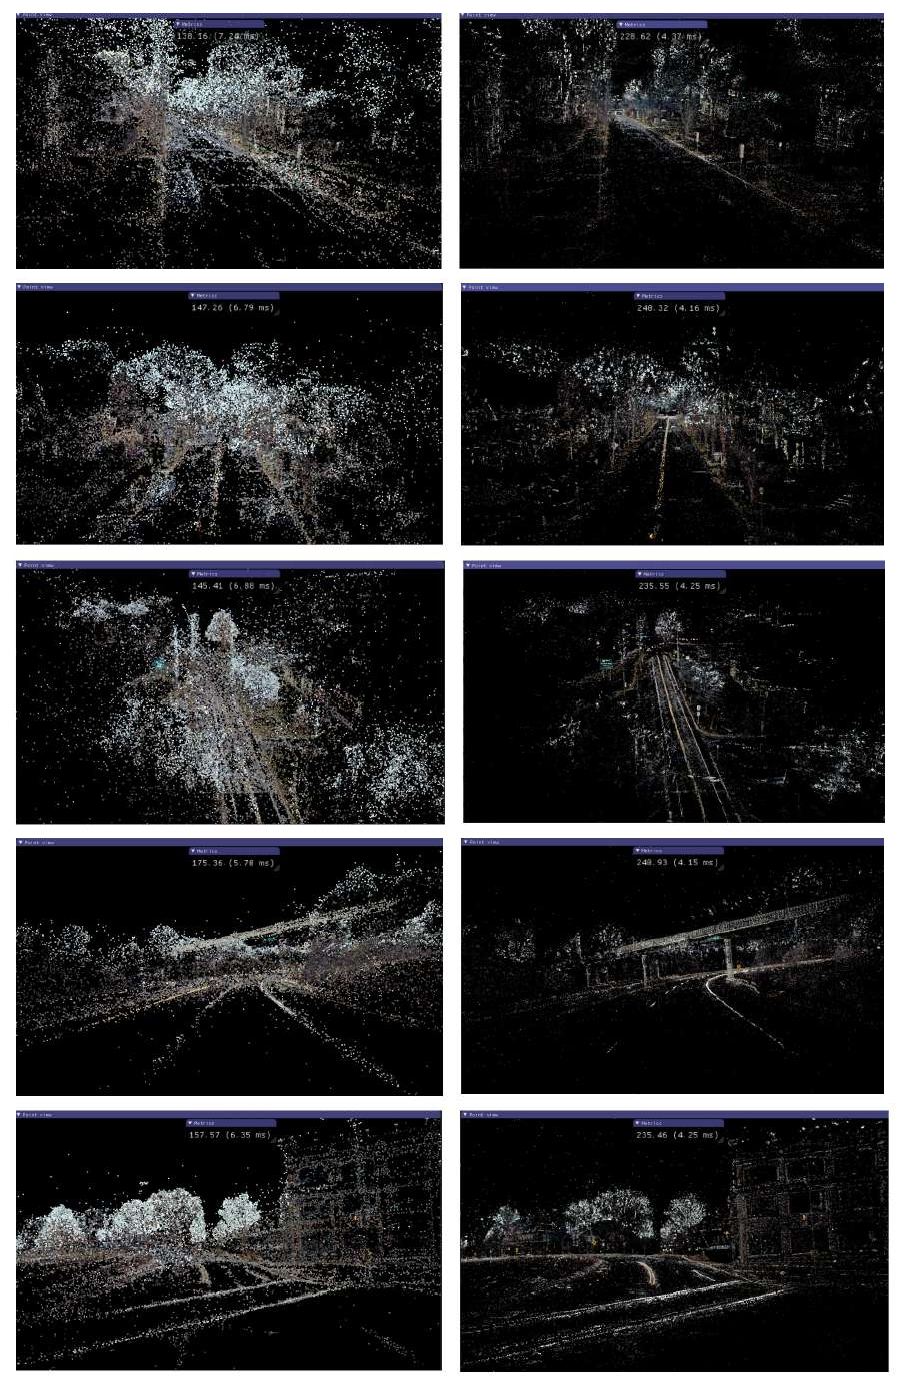
\includegraphics[width=0.8\linewidth]{figs_compressed/reconstruction_compressed.pdf}
    \caption{\textbf{Left: SfM Initialized Points. Right: Gaussian Points after Optimization.}}
    \label{fig:reconstruction-appendix}
\end{figure}


\begin{figure}[ht]
    \centering
    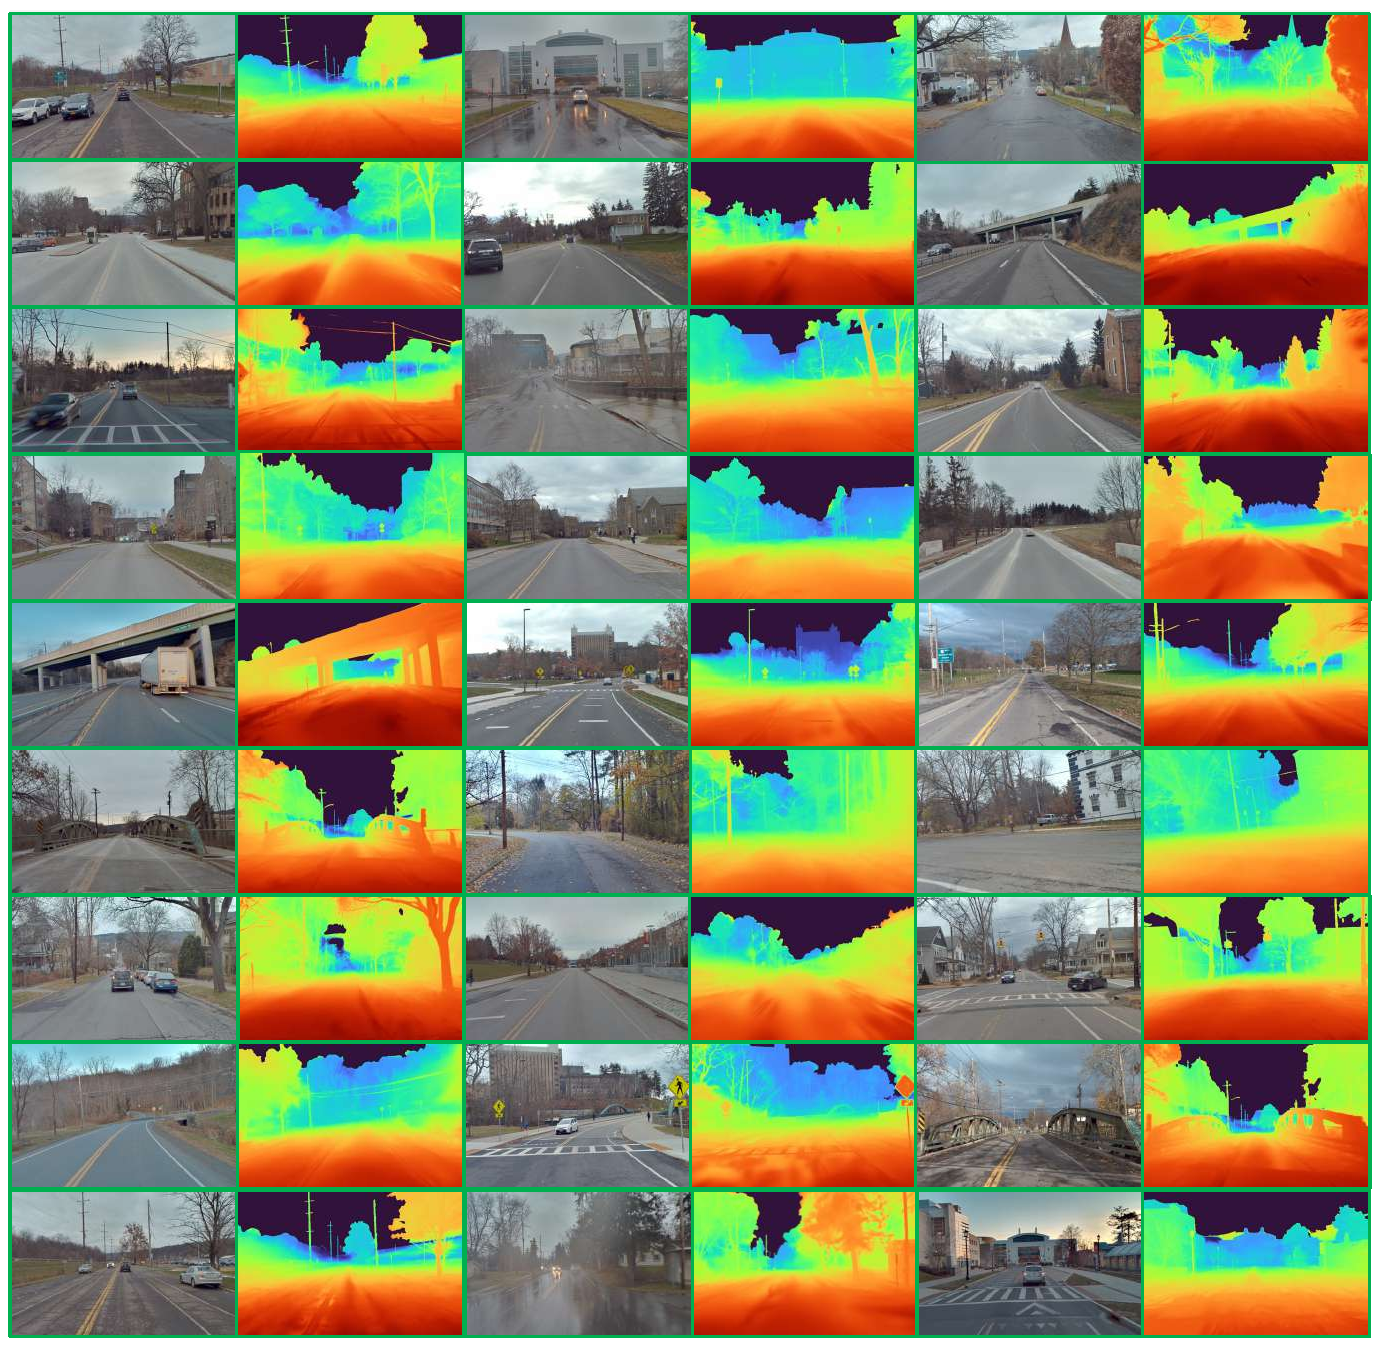
\includegraphics[width=\linewidth]{figs_compressed/ithaca-depth-app_compressed.pdf}
    \caption{\textbf{Visualizations of depth images in Mapverse-Ithaca365}}
    \label{fig:ithaca-depth-appendix}
\end{figure}


\clearpage


\section{Mapverse-Ithaca365: Additional Visualizations of Neural Rendering}

\begin{figure}[ht]
\begin{center}
\centerline{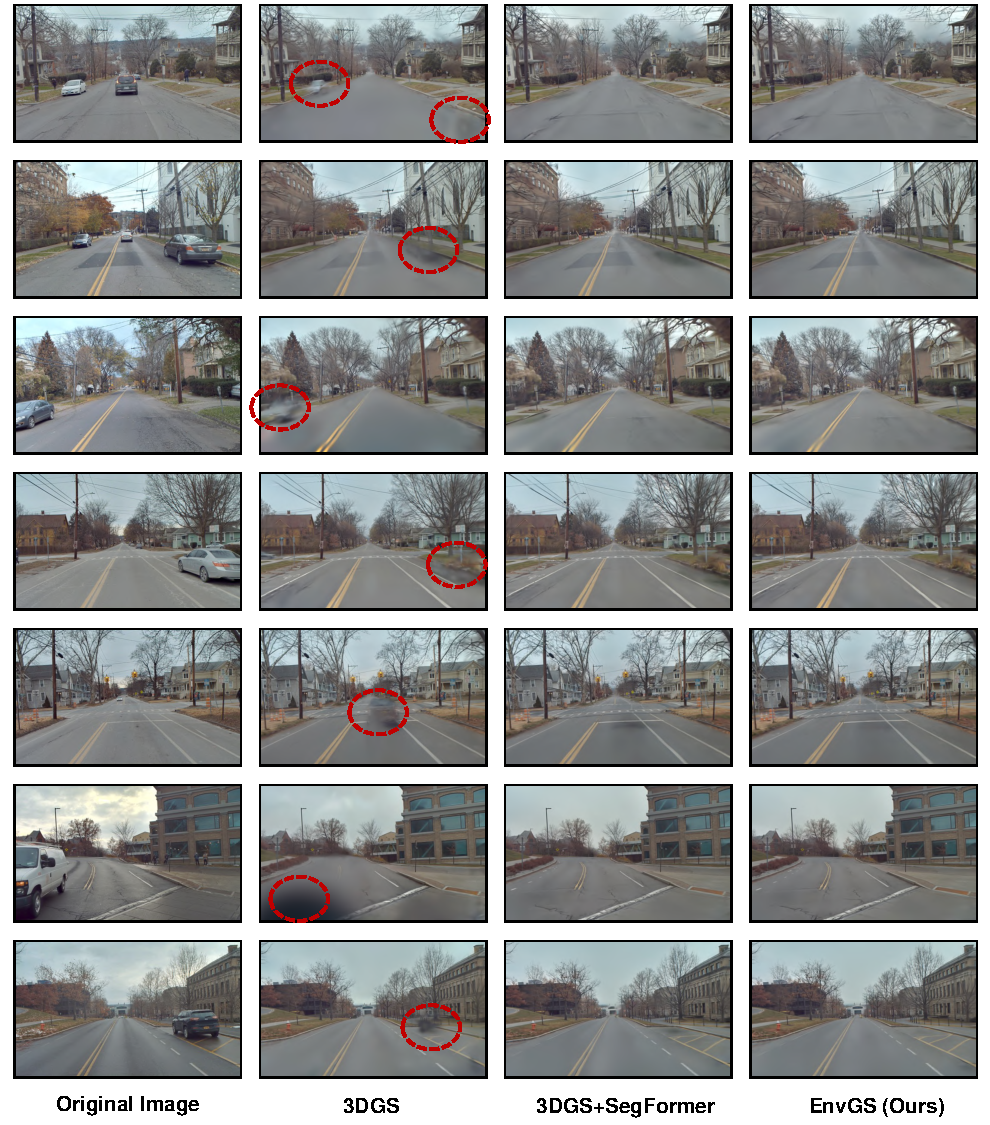
\includegraphics[width=\columnwidth]{figs_compressed/envrendering-supp_compressed.pdf}}
\caption{\textbf{Qualitative evaluations of the environment rendering.} Our method demonstrates robust performance against transient objects.}
\label{fig:rendering-appendix}
\end{center}
\vspace{-10mm}
\end{figure}


\clearpage


\section{Mapverse-nuPlan: Unsupervised 2D Segmentation}
\label{sec:seg-nuplan-app}
\subsection{Quantitative Results}

We employ SegFormer~\cite{xie2021segformer} to generate pseudo ground-truth masks and compare these with the output of \texttt{EmerSeg} using Intersection over Union (IoU) metrics in Mapverse-nuPlan collected in Las Vegas. Figure~\ref{fig:iouvsloc-nuplan} displays the IoU scores across different locations. The highest IoU score is at loc6 with 59.53\%, indicating the best segmentation performance. In contrast, loc20 has the lowest score at 28.69\%, indicating the poorest performance. \textbf{The average IoU score across all locations is approximately 46.51\%}, which surpasses the IoU score of 45.14\% on Mapverse-Ithaca365. Las Vegas is known for its dense traffic and complex urban environment compared to Ithaca, which presents a different set of challenges for segmentation models. The improved performance in the more demanding Las Vegas environment indicates that \texttt{EmerSeg} can \textit{adapt to various traffic densities and urban complexities}, maintaining high accuracy without requiring extensive parameter tuning.

The variation in IoU scores across different locations can be attributed to several factors, including the complexity of the scene, lighting conditions, and the presence of occlusions. Locations with higher IoU scores, such as loc6, likely benefit from clearer images and less occlusion, allowing for more accurate segmentation. Conversely, locations like loc20, with lower IoU scores, may suffer from challenging conditions such as poor lighting and complex backgrounds.




\begin{figure}[ht]
    \centering
    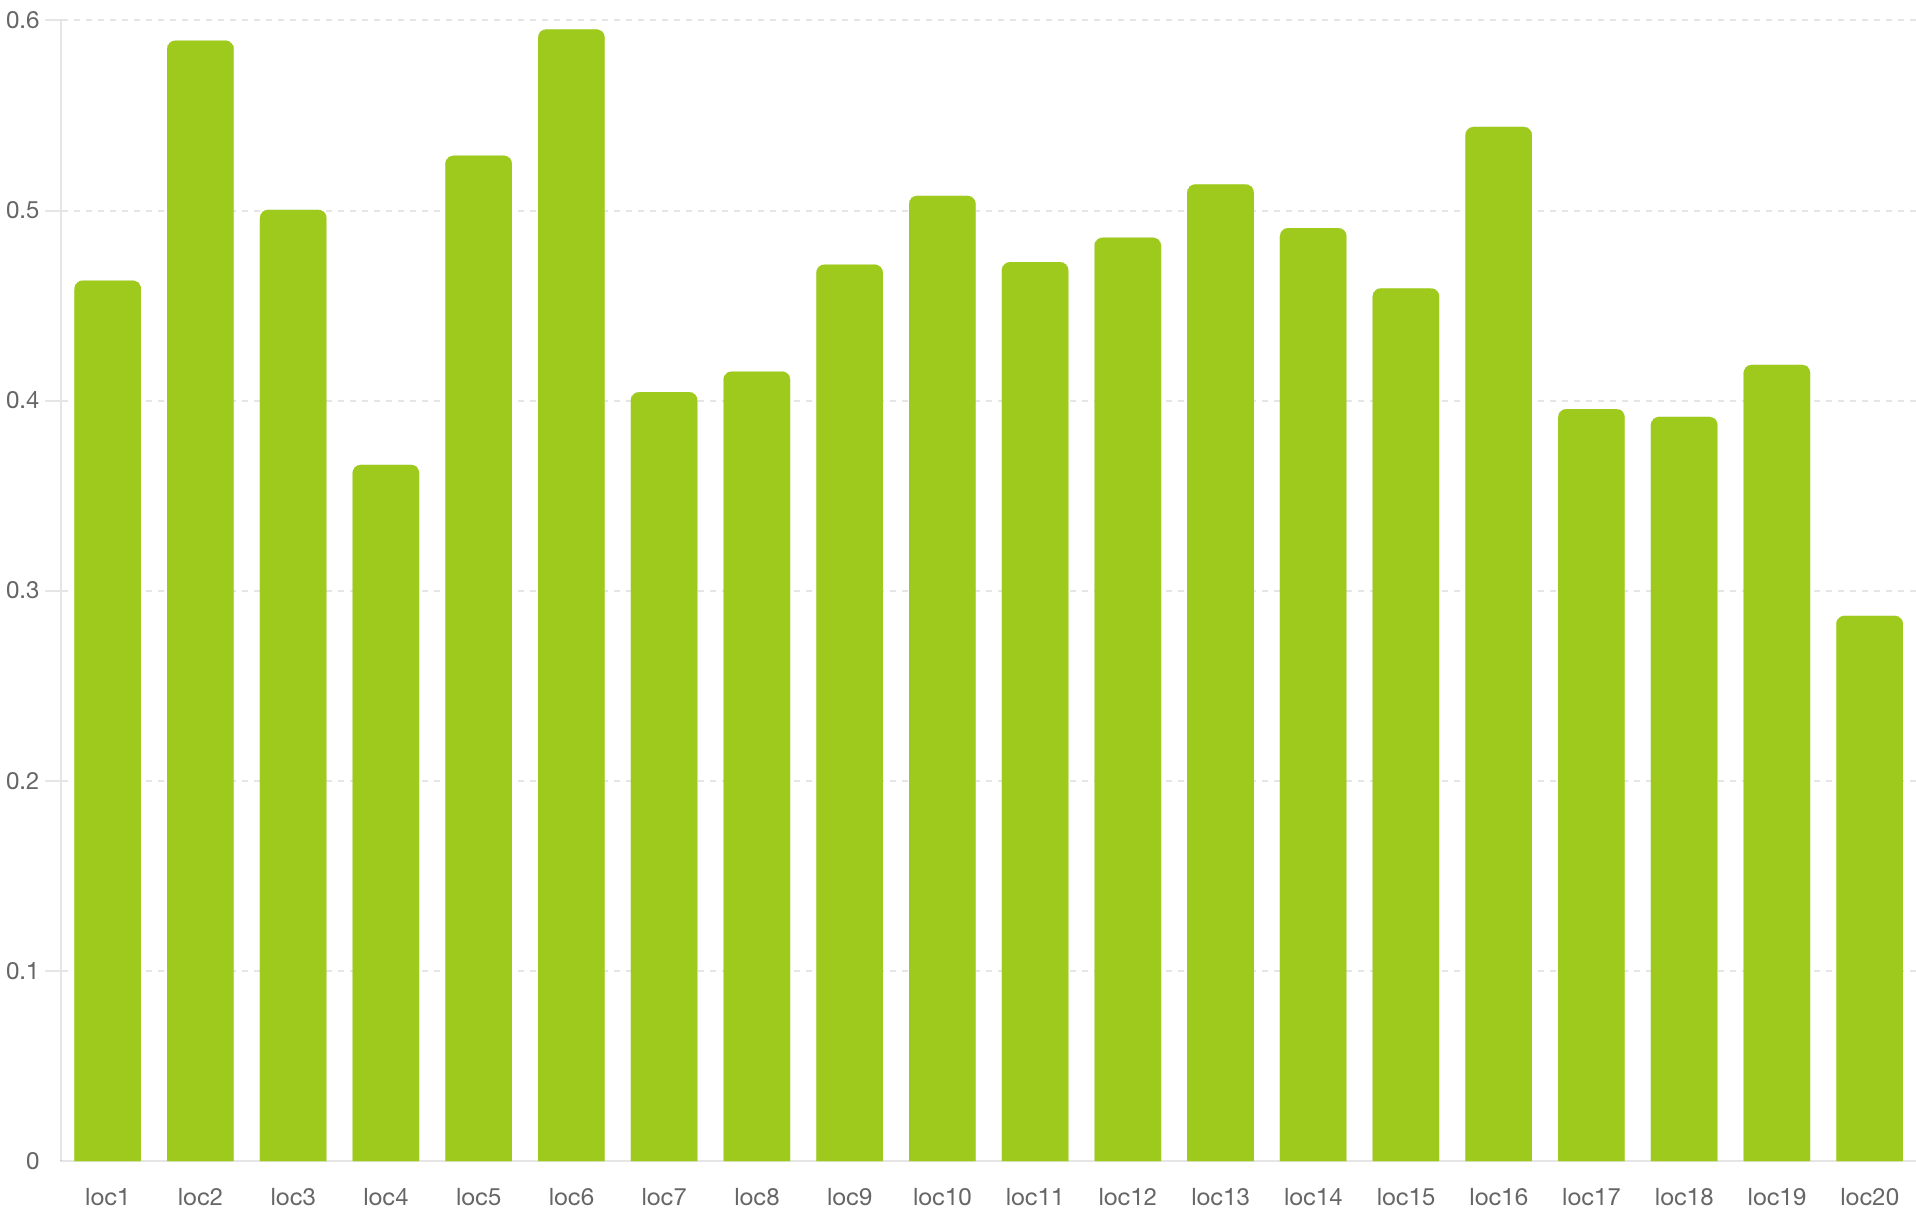
\includegraphics[width=\linewidth]{figs_compressed/nuplan-iou-locations.png}
    \caption{\textbf{IoU of \texttt{EmerSeg} compared to SegFormer across locations in Mapverse-nuPlan.}}
    \label{fig:iouvsloc-nuplan}
\end{figure}


\subsection{Qualitative Results}
We visualize some segmentation results in Fig.\ref{fig:vegas-loc1} to Fig.\ref{fig:vegas-loc6}. The visualizations highlight \texttt{EmerSeg}'s ability to accurately segment objects in complex traffic situations with multiple dynamic elements. These results underscore the versatility and reliability of our approach, showcasing its potential for real-world applications in autonomous driving and other vision-based tasks.

\begin{figure}[ht]
    \centering
    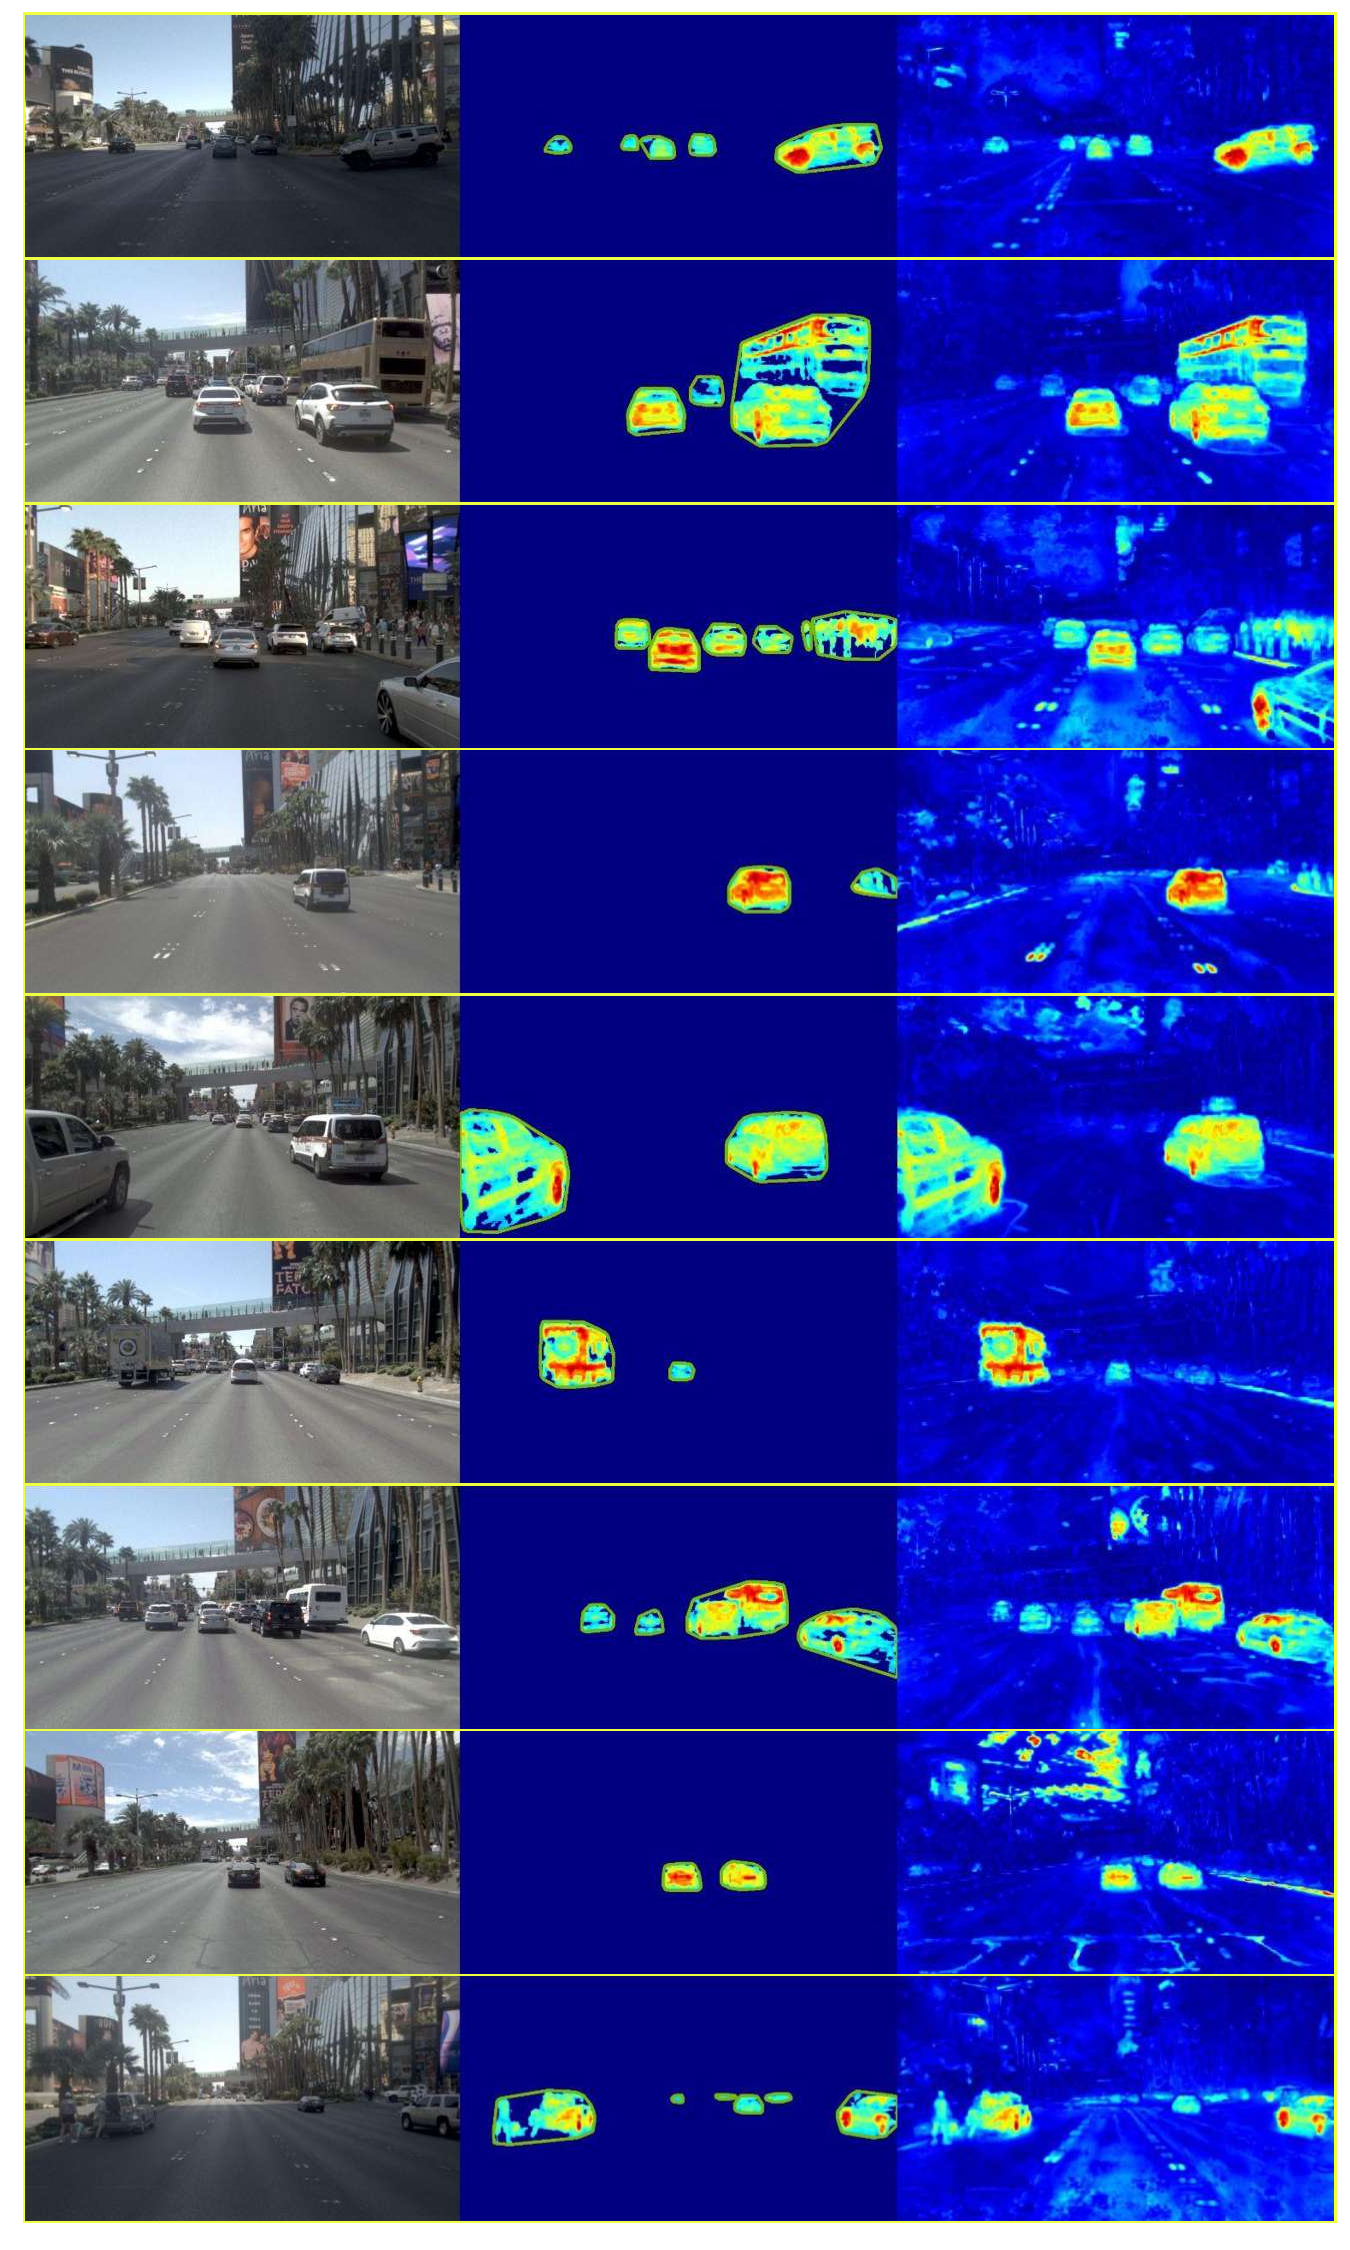
\includegraphics[width=0.88\linewidth]{figs_compressed/EmerSeg-loc1_compressed.pdf}
    \caption{\textbf{Qualitative results of \texttt{EmerSeg} for multiple traversals of location 1 of Mapverse-nuPlan.} From left to right: raw RGB image, extracted 2D ephemeral object masks, and normalized feature residuals visualized using a jet color map.}
    \label{fig:vegas-loc1}
\end{figure}

\begin{figure}[ht]
    \centering
    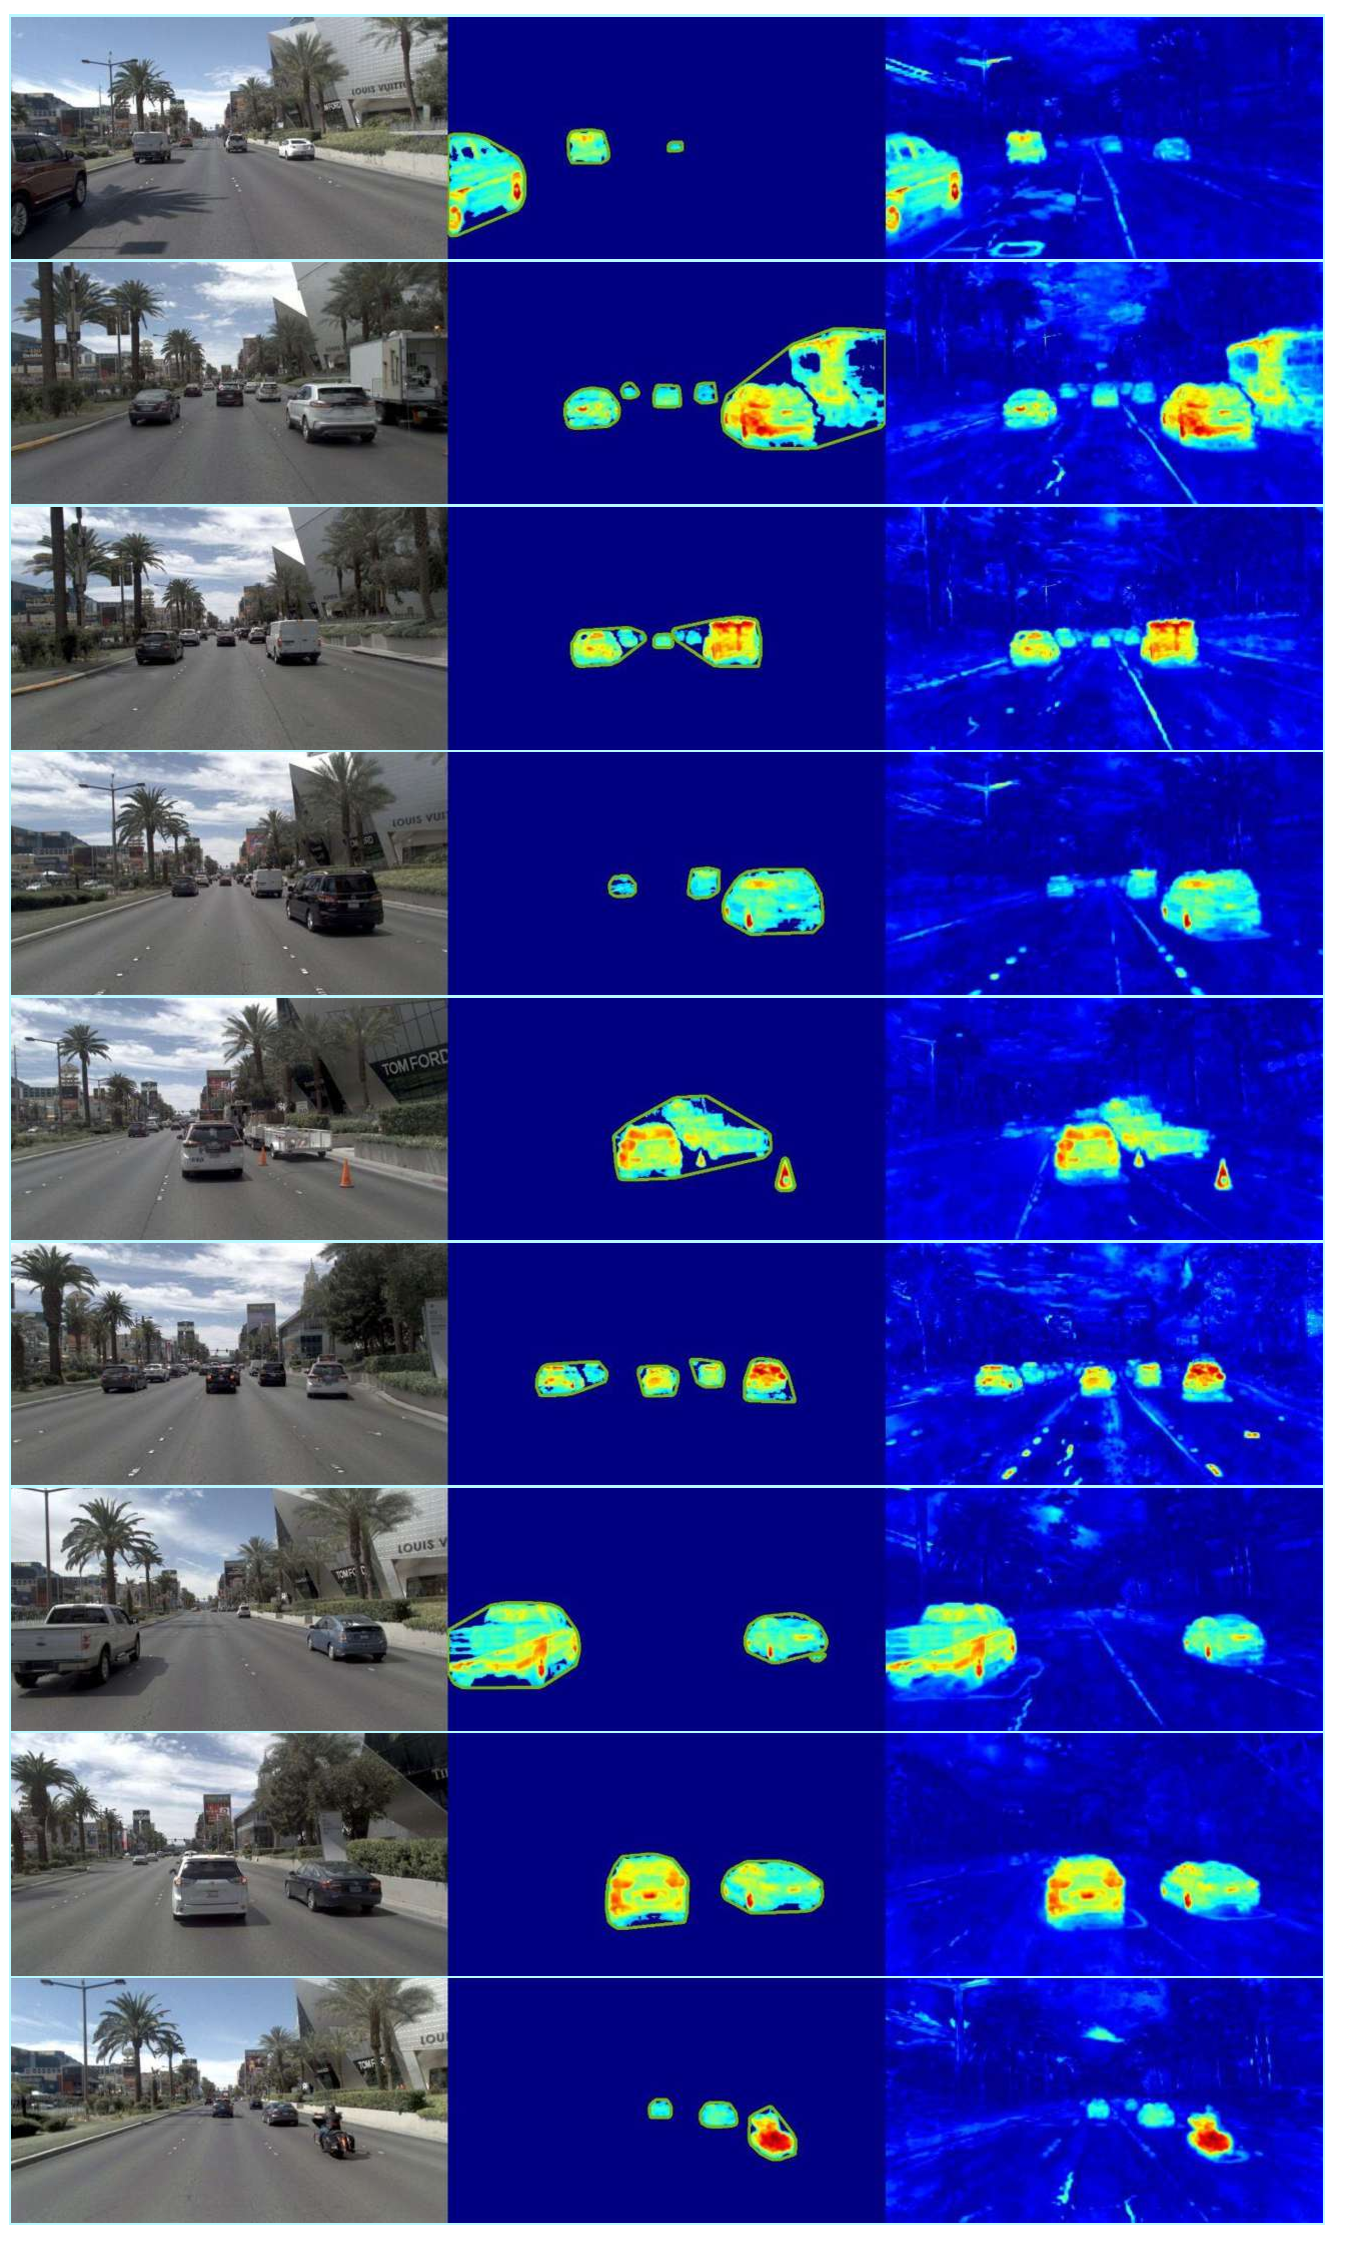
\includegraphics[width=0.88\linewidth]{figs_compressed/EmerSeg-loc2_compressed.pdf}
    \caption{\textbf{Qualitative results of \texttt{EmerSeg} for multiple traversals of location 2 of Mapverse-nuPlan.} From left to right: raw RGB image, extracted 2D ephemeral object masks, and normalized feature residuals visualized using a jet color map.}
    \label{fig:vegas-loc2}
\end{figure}

\begin{figure}[ht]
    \centering
    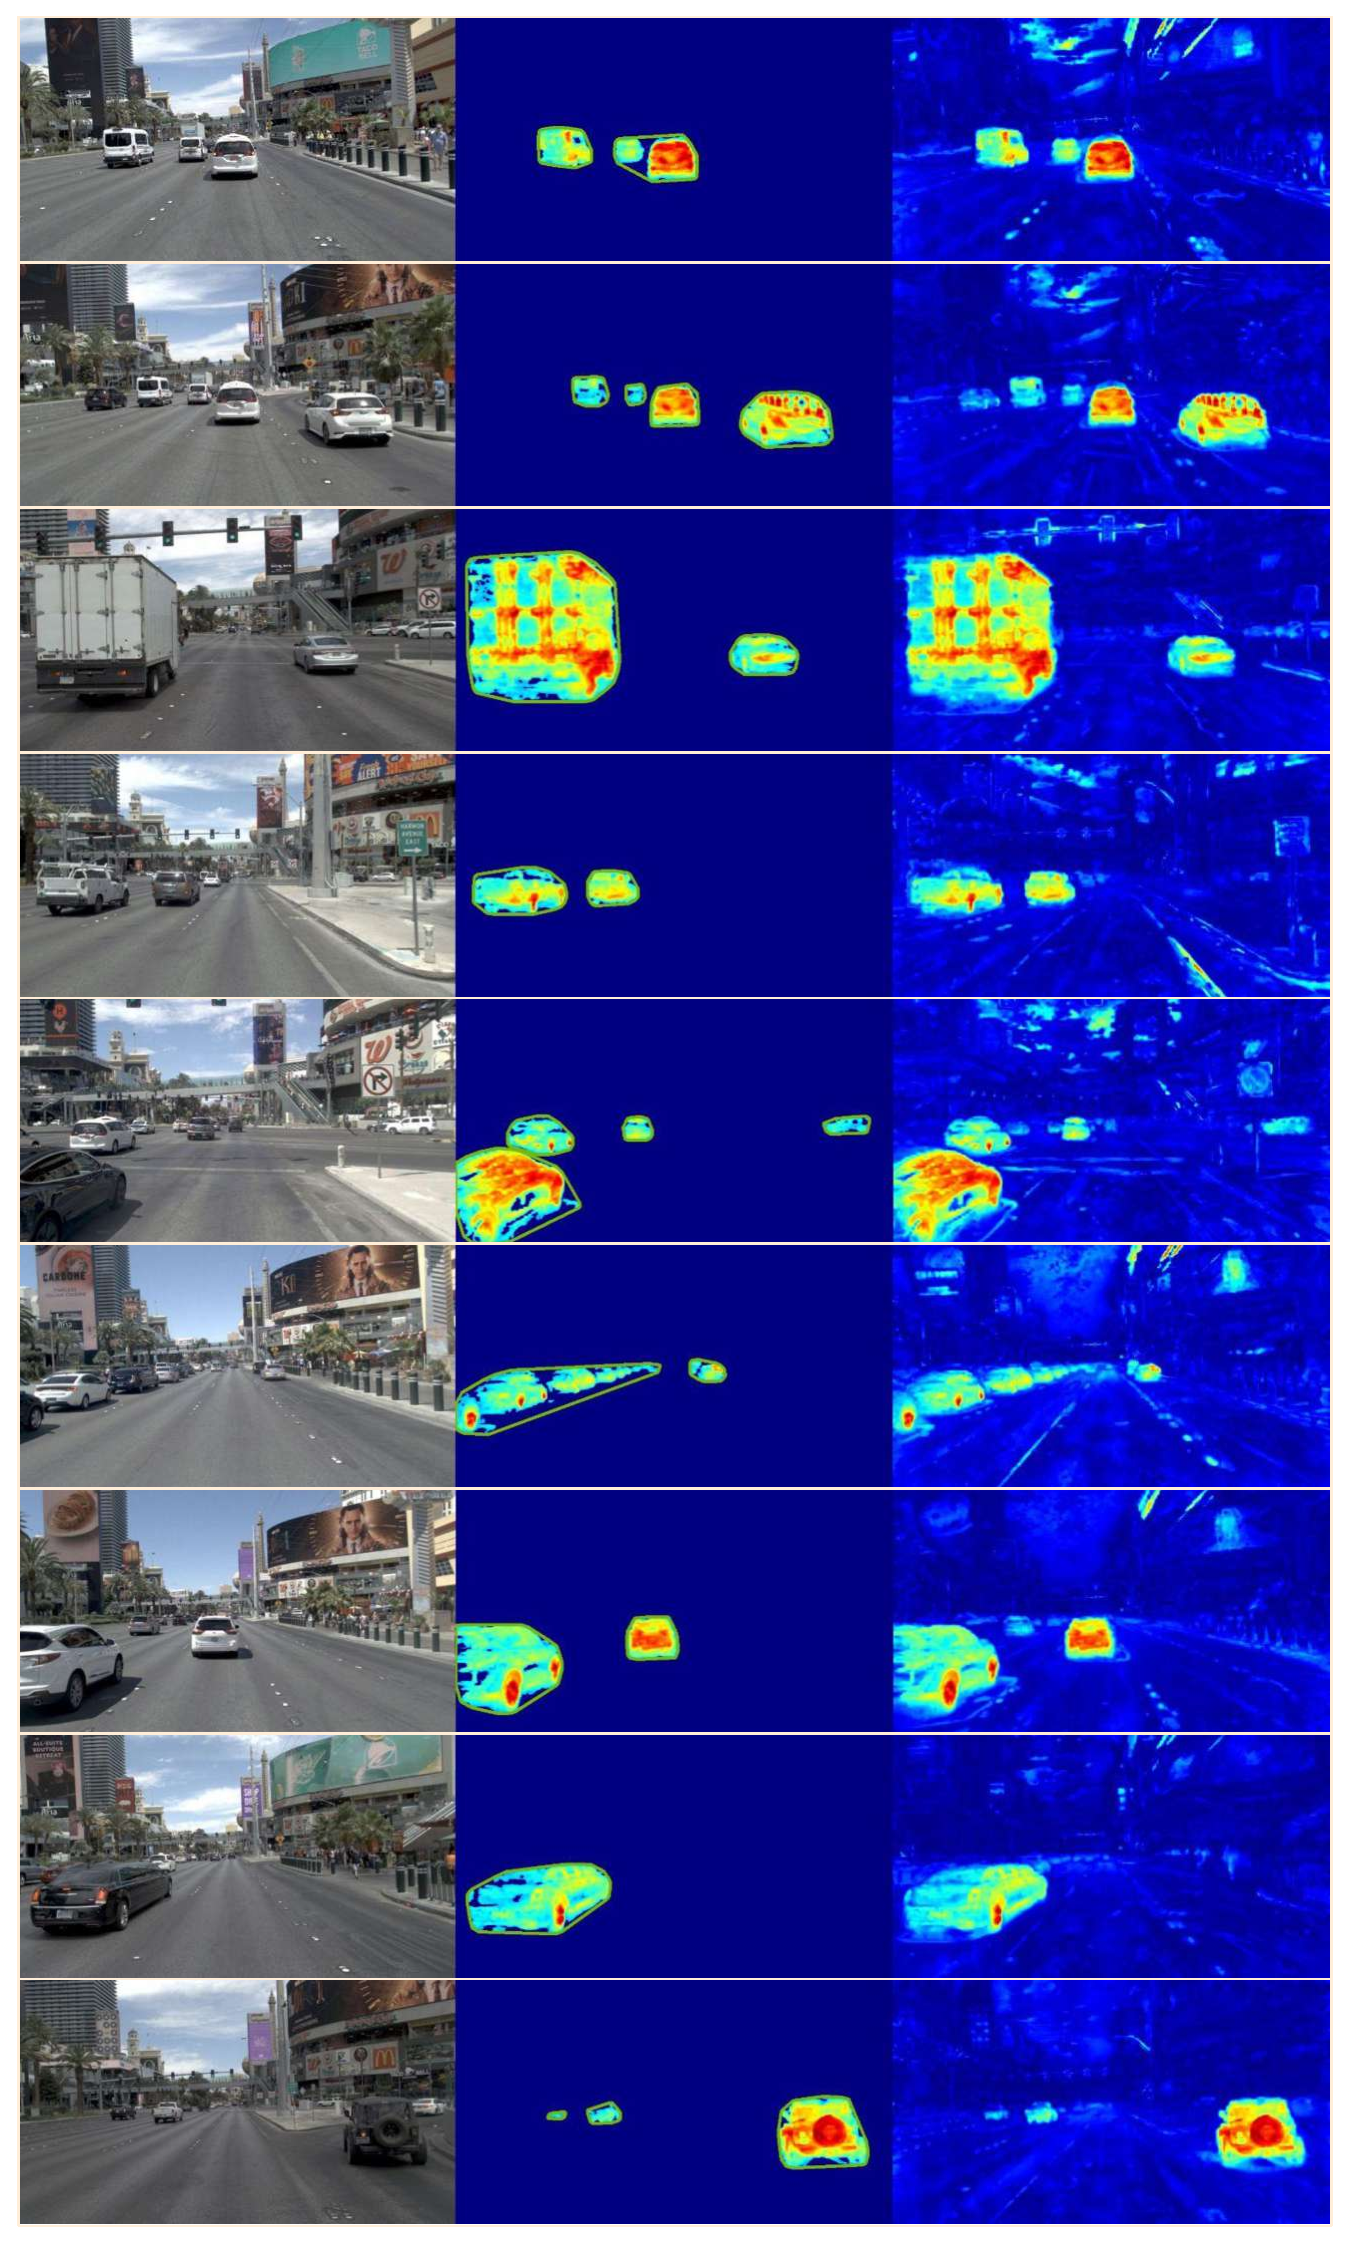
\includegraphics[width=0.88\linewidth]{figs_compressed/EmerSeg-loc3_compressed.pdf}
    \caption{\textbf{Qualitative results of \texttt{EmerSeg} for multiple traversals of location 3 of Mapverse-nuPlan.} From left to right: raw RGB image, extracted 2D ephemeral object masks, and normalized feature residuals visualized using a jet color map.}
    \label{fig:vegas-loc3}
\end{figure}

\begin{figure}[ht]
    \centering
    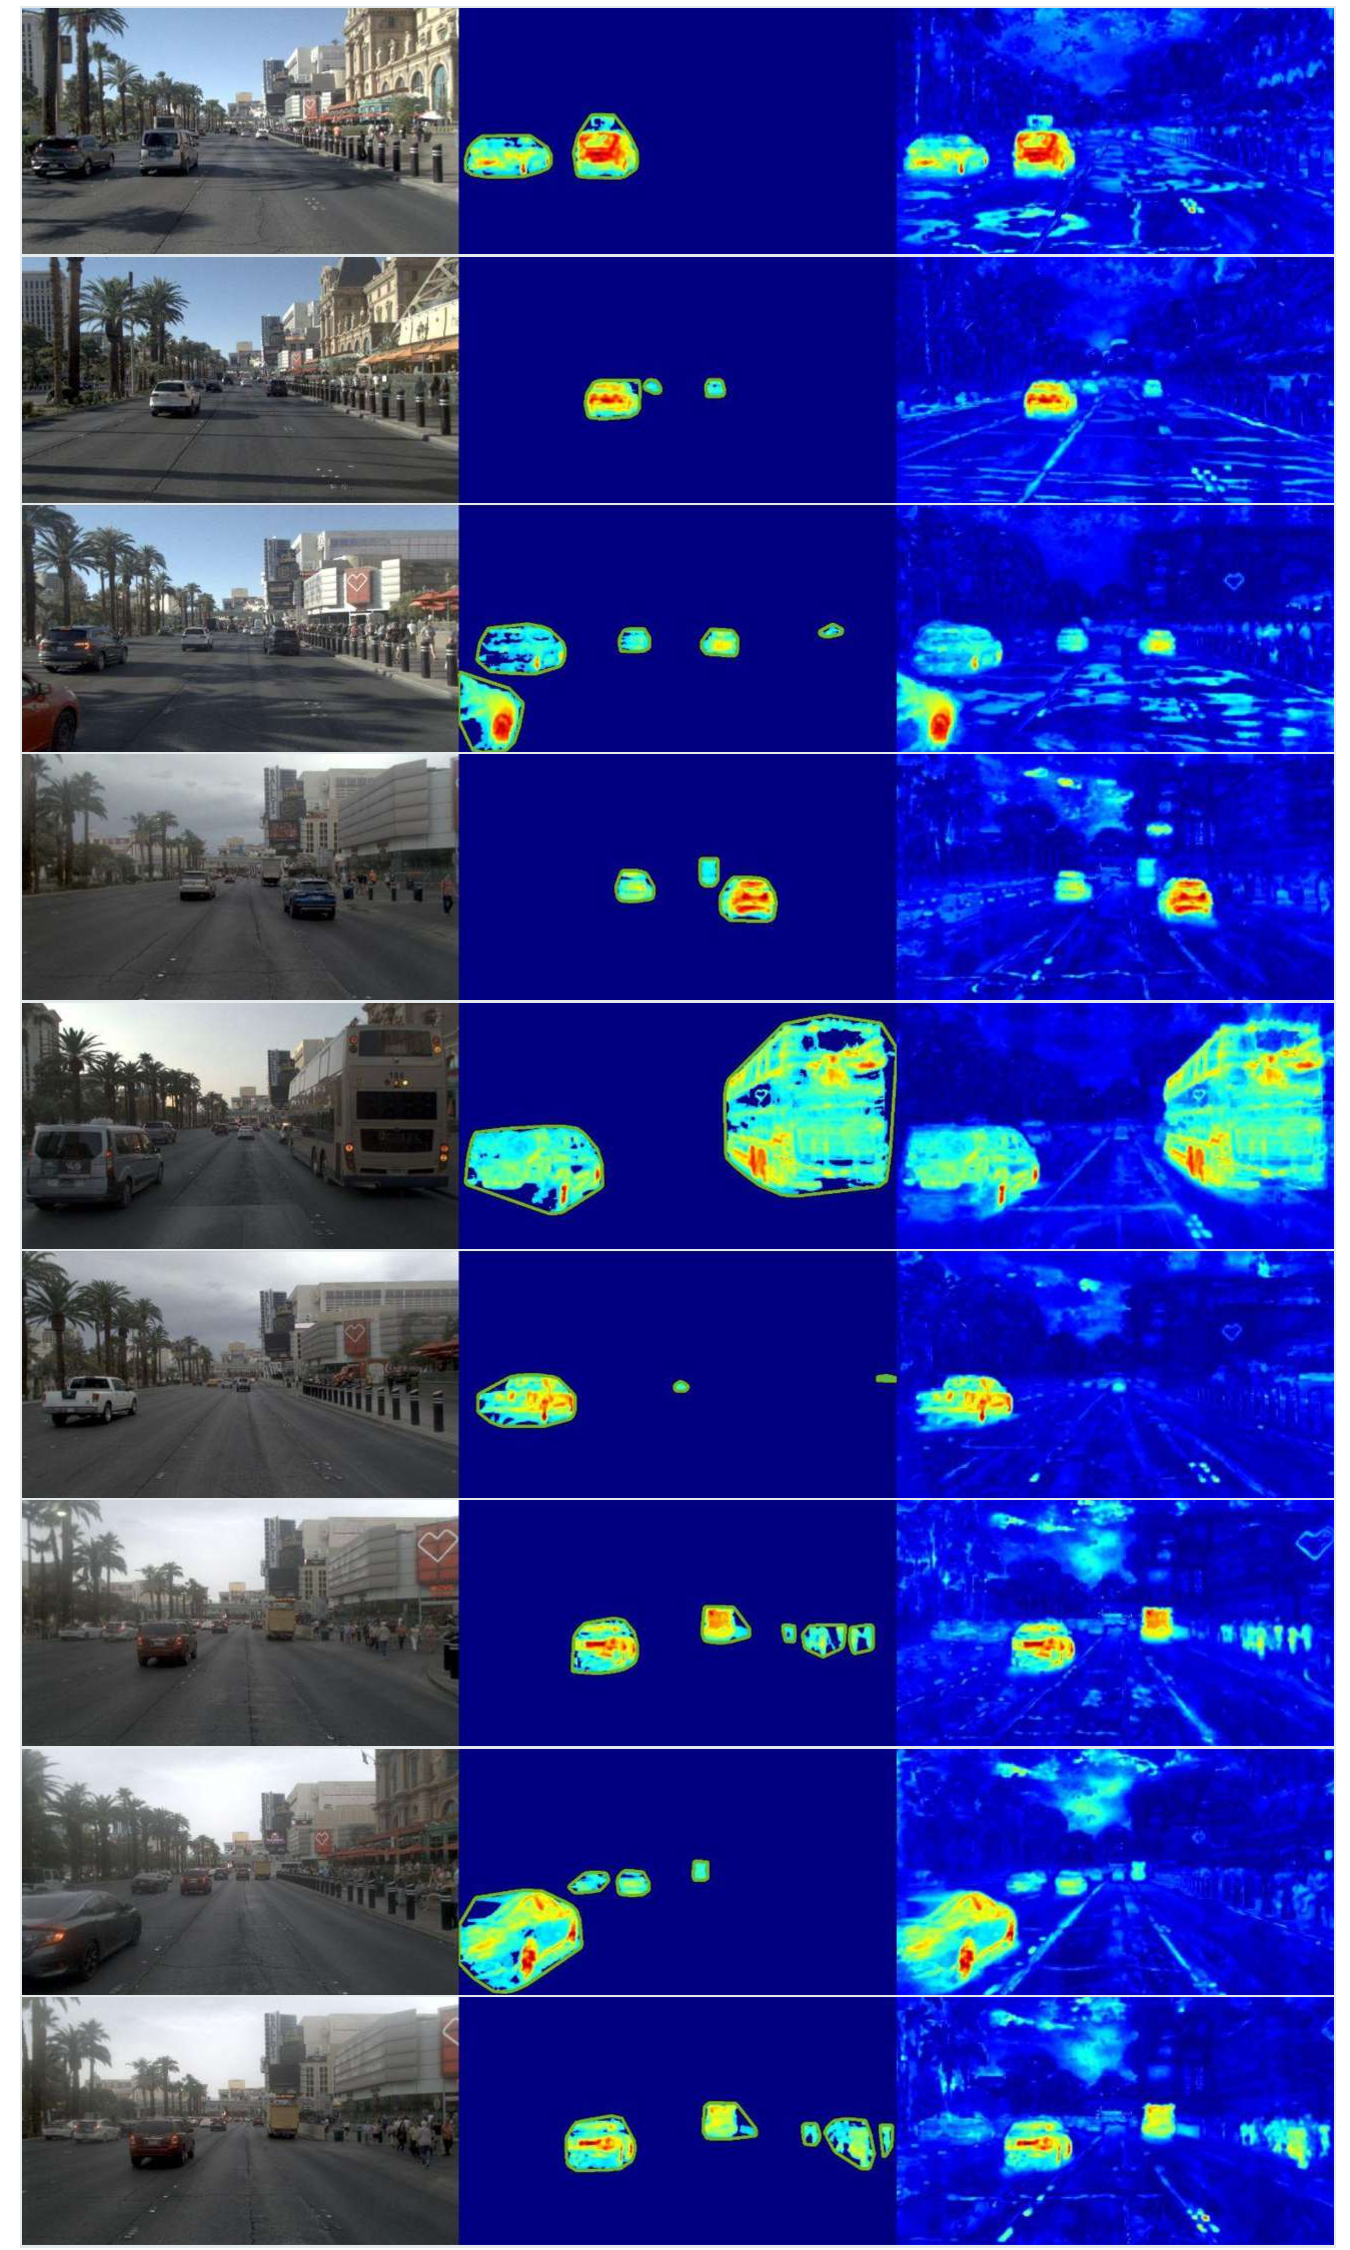
\includegraphics[width=0.88\linewidth]{figs_compressed/EmerSeg-loc4_compressed.pdf}
    \caption{\textbf{Qualitative results of \texttt{EmerSeg} for multiple traversals of location 4 of Mapverse-nuPlan.} From left to right: raw RGB image, extracted 2D ephemeral object masks, and normalized feature residuals visualized using a jet color map.}
    \label{fig:vegas-loc4}
\end{figure}

\begin{figure}[ht]
    \centering
    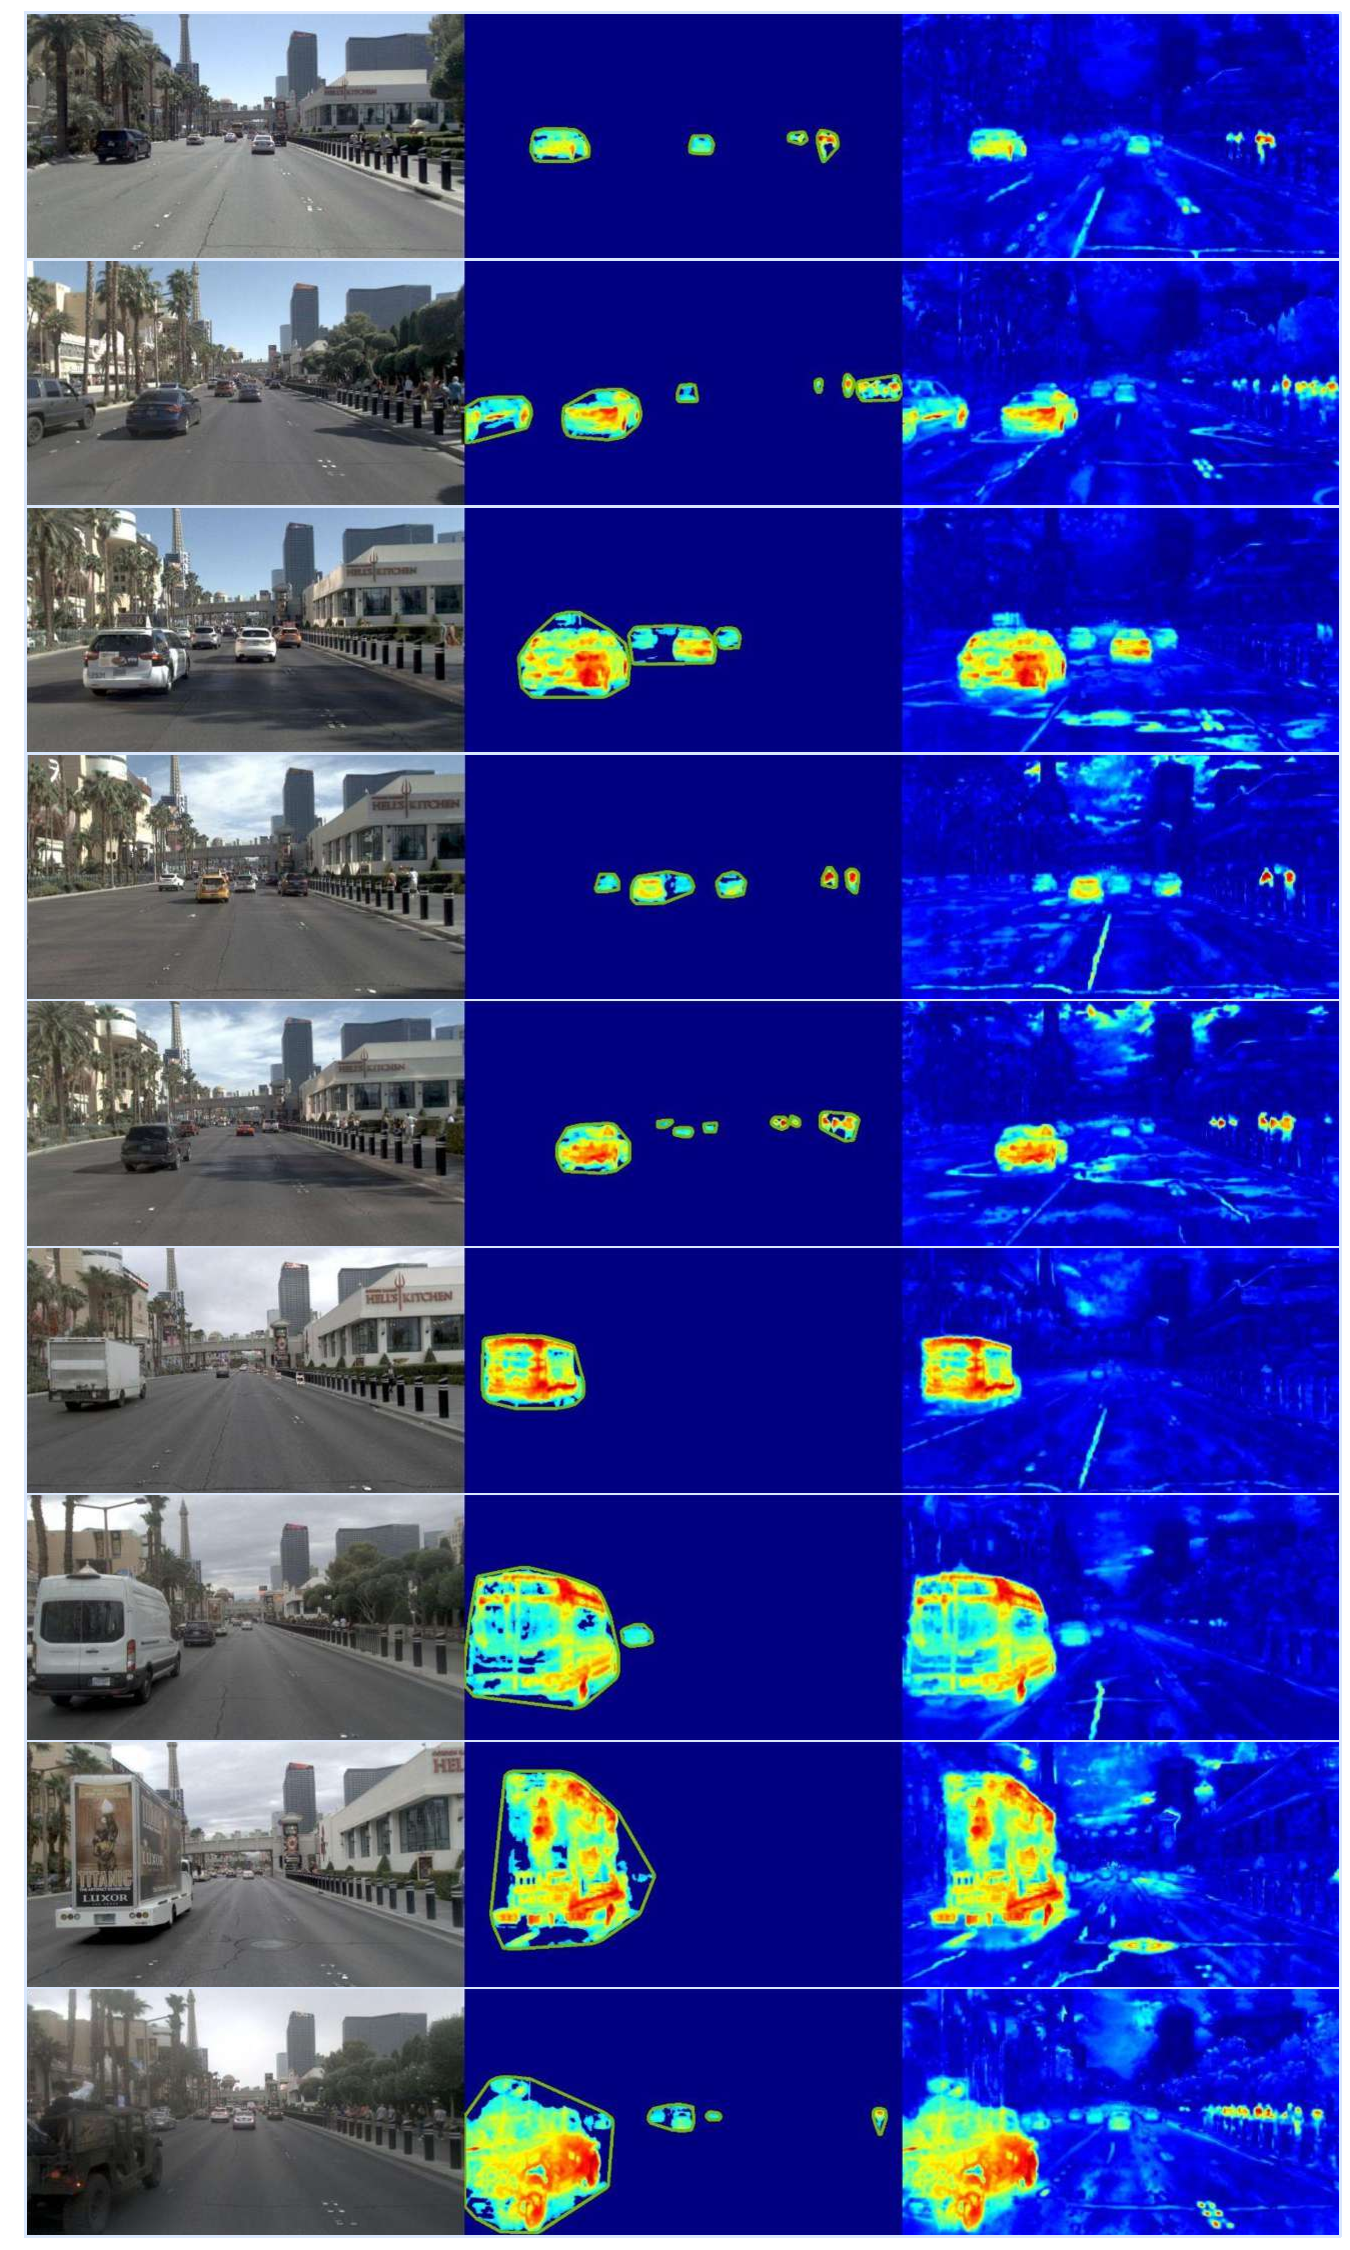
\includegraphics[width=0.88\linewidth]{figs_compressed/EmerSeg-loc5_compressed.pdf}
    \caption{\textbf{Qualitative results of \texttt{EmerSeg} for multiple traversals of location 5 of Mapverse-nuPlan.} From left to right: raw RGB image, extracted 2D ephemeral object masks, and normalized feature residuals visualized using a jet color map.}
    \label{fig:vegas-loc5}
\end{figure}

\begin{figure}[ht]
    \centering
    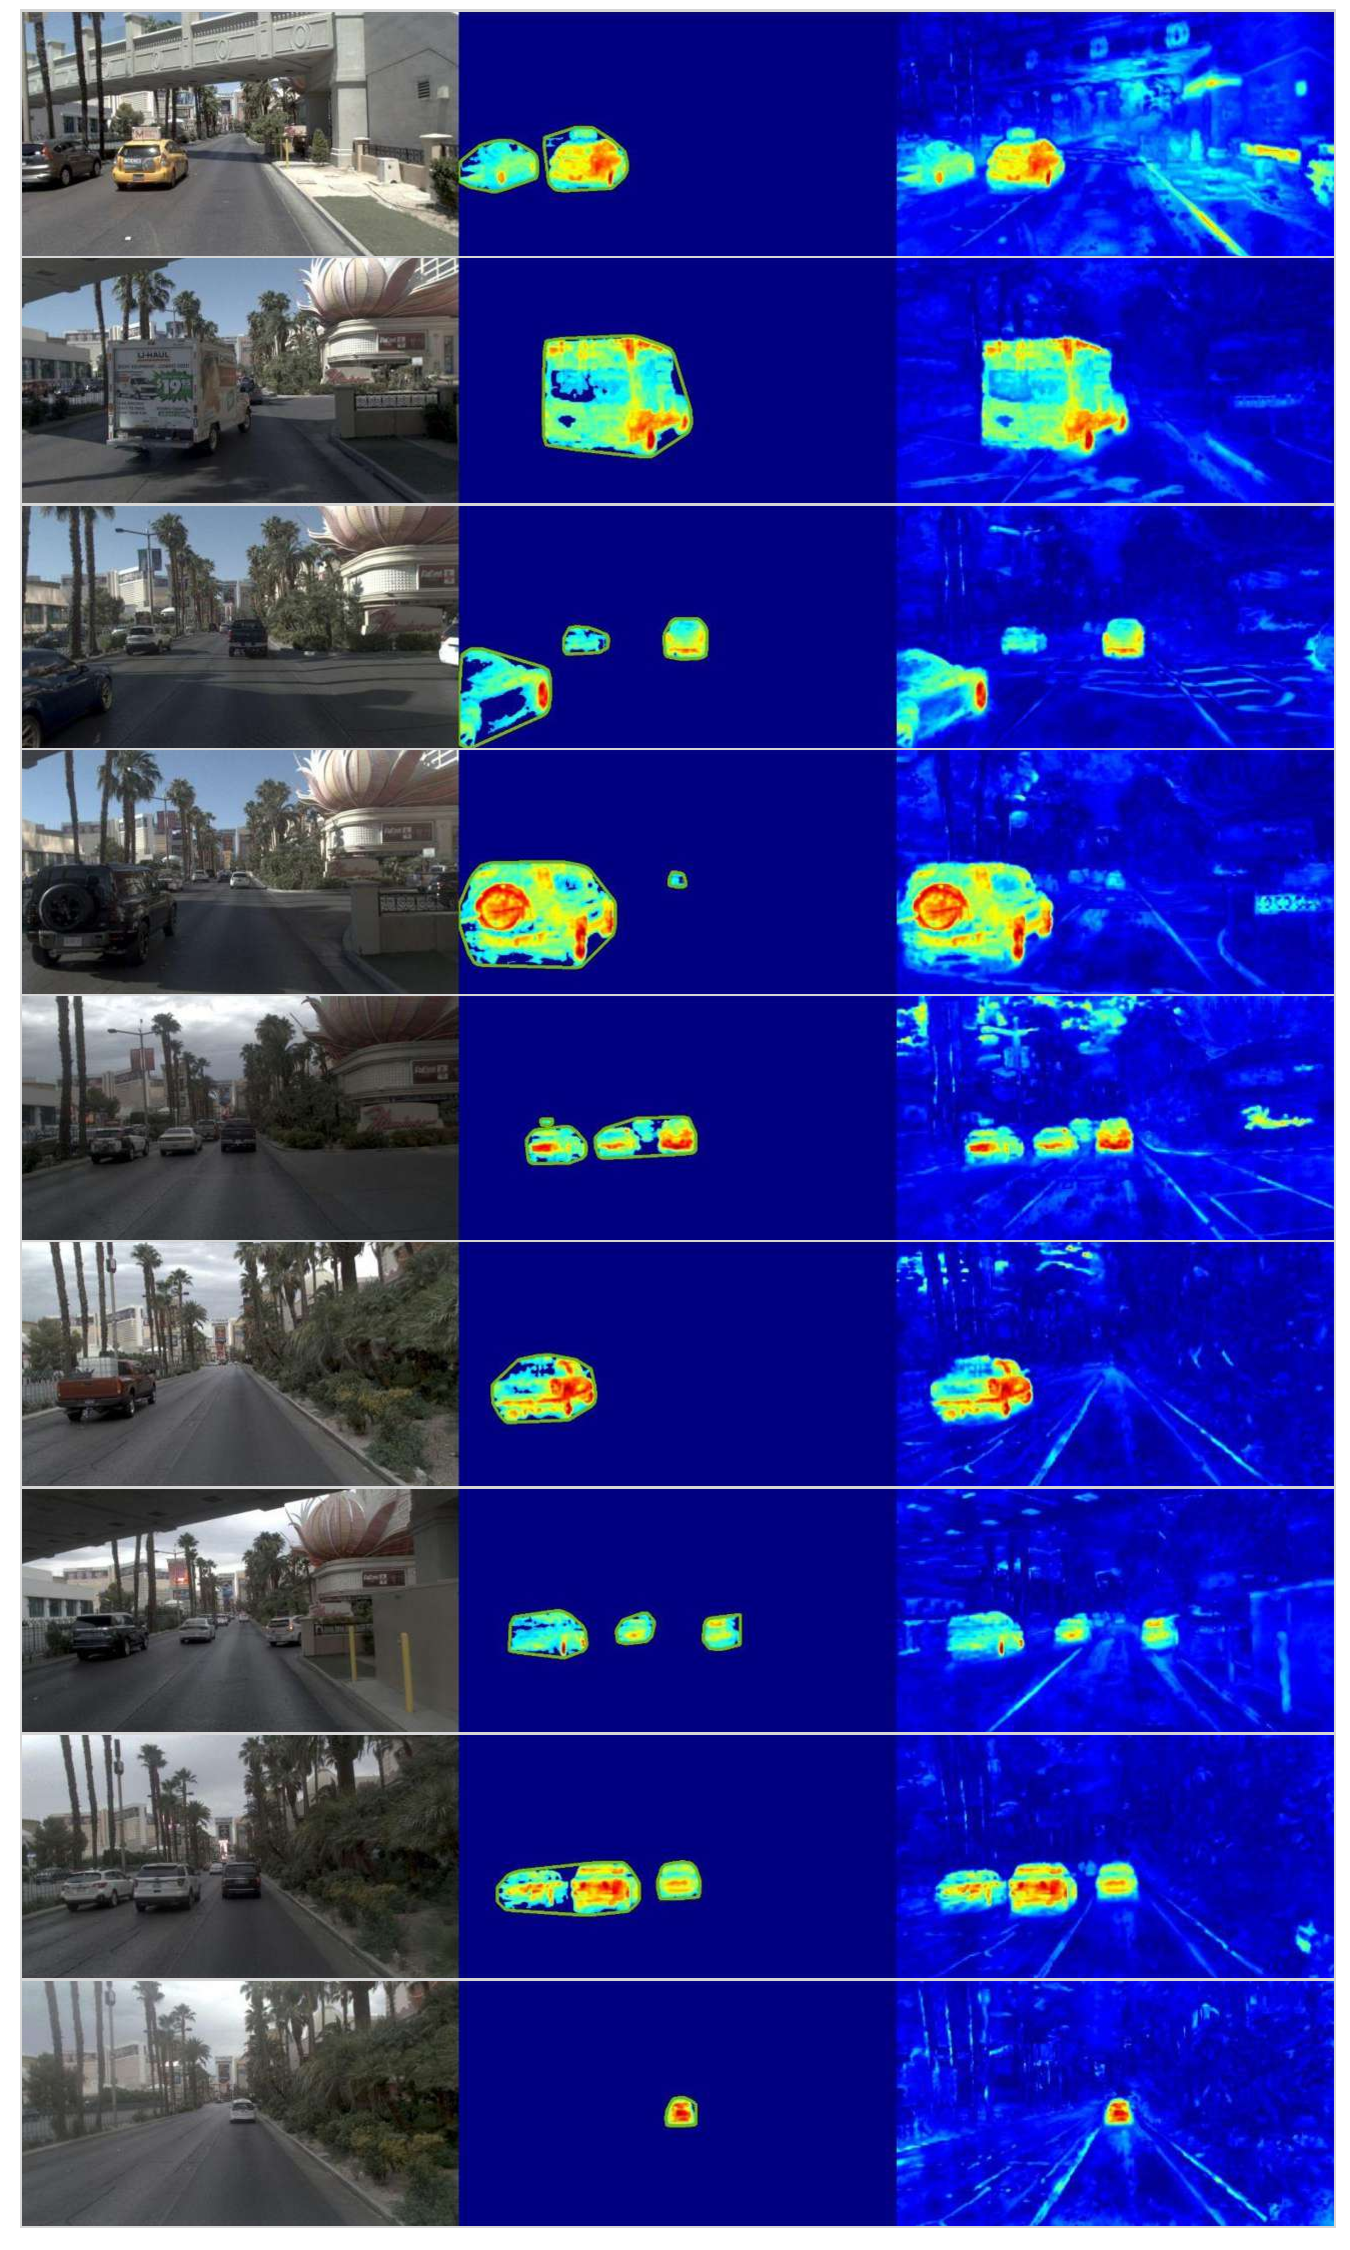
\includegraphics[width=0.88\linewidth]{figs_compressed/EmerSeg-loc6_compressed.pdf}
    \caption{\textbf{Qualitative results of \texttt{EmerSeg} for multiple traversals of location 6 of Mapverse-nuPlan.} From left to right: raw RGB image, extracted 2D ephemeral object masks, and normalized feature residuals visualized using a jet color map.}
    \label{fig:vegas-loc6}
\end{figure}



\clearpage
\section{Mapverse-nuPlan: Depth Visualization}
\label{sec:depth-nuplan-app}

\begin{figure}[ht]
\vspace{10mm}
    \centering
    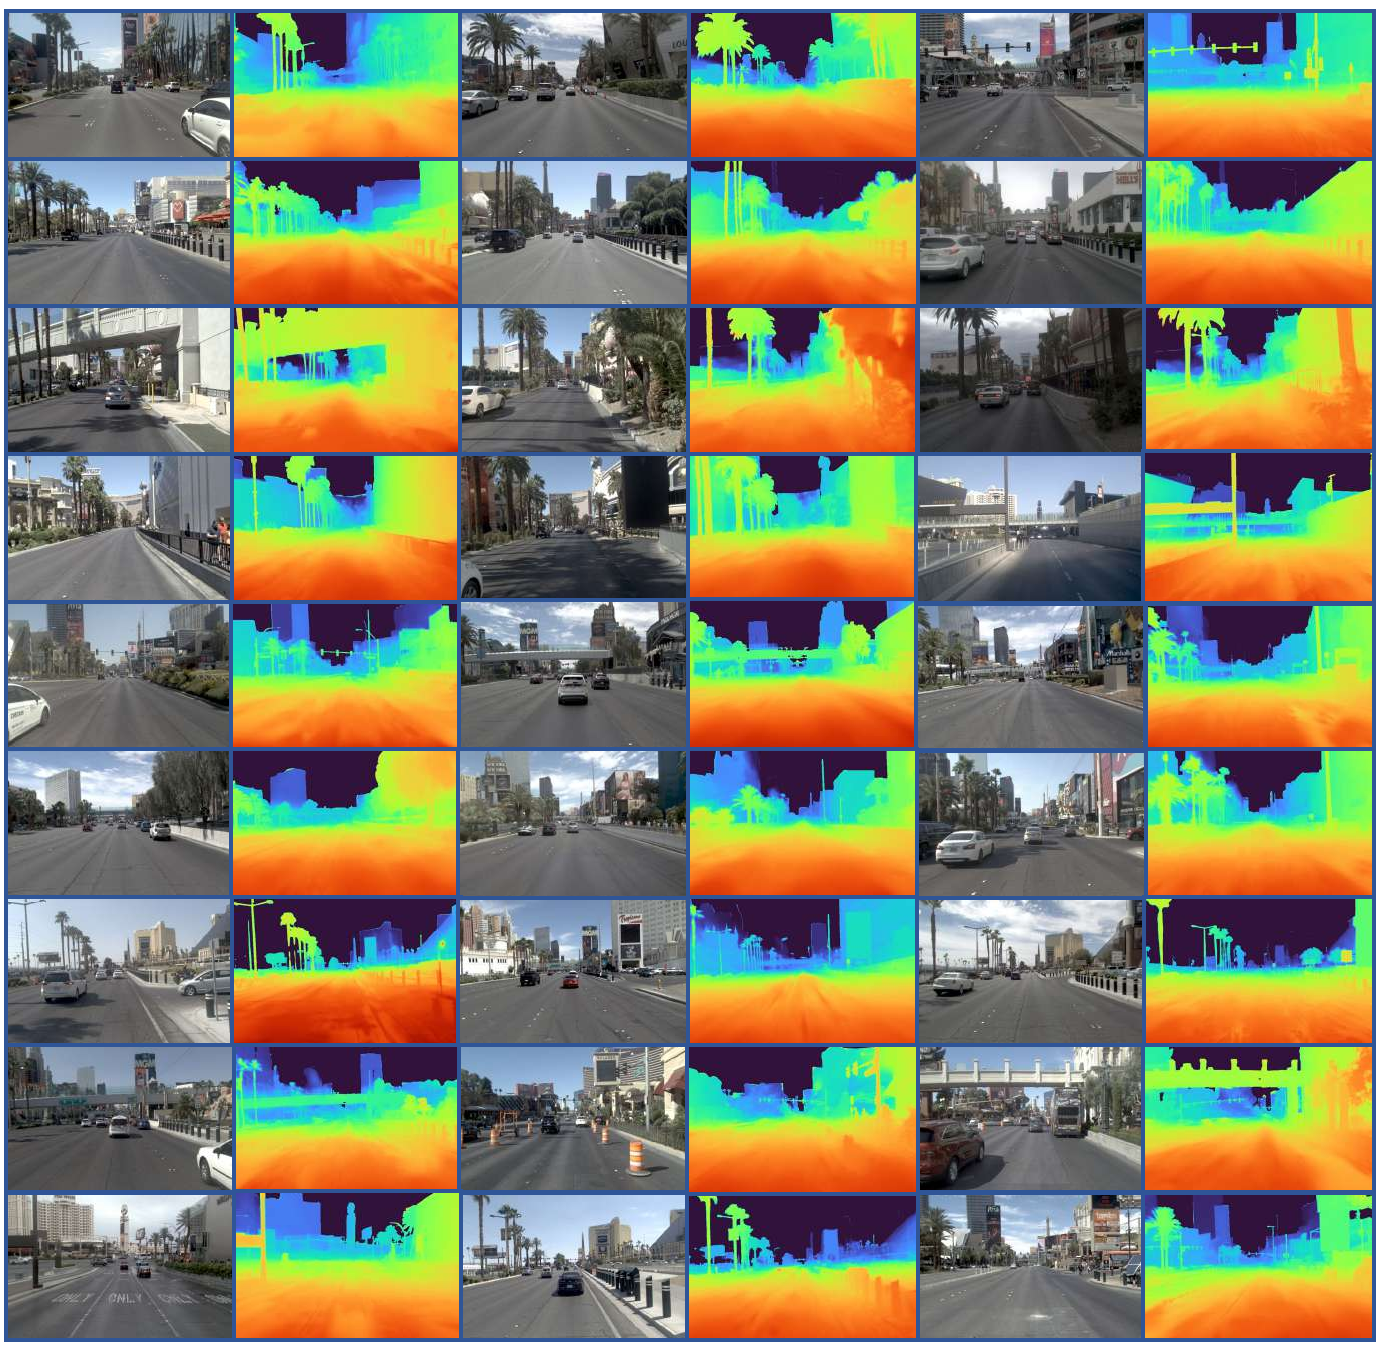
\includegraphics[width=\linewidth]{figs_compressed/nuplan-depth-app_compressed.pdf}
    \caption{\textbf{Visualizations of depth images in Mapverse-Ithaca365}}
    \label{fig:nuplan-depth-appendix}
\end{figure}


\clearpage
\section{Mapverse-nuPlan: Neural Rendering}
\label{sec:rendering-nuplan-app}

% Please add the following required packages to your document preamble:
% \usepackage{booktabs}
% \usepackage{multirow}
\begin{table}[ht]
\scriptsize
\centering
\caption{\textbf{Quantitative rendering results in Mapverse-nuPlan.} We set test/training views as 1/8. Pixels corresponding to transient objects are removed in the evaluations since we do not have ground truth background pixels in these regions occluded by transient objects.}
\begin{tabular}{@{}c|ccc|ccc|ccc@{}}
\toprule
\multirow{2}{*}{\textbf{Location}} & \multicolumn{3}{c|}{\textbf{3DGS}}                                 & \multicolumn{3}{c|}{\textbf{3DGS+SegFormer}}                      & \multicolumn{3}{c}{\textbf{EnvGS (Ours)}}                                 \\ \cmidrule(l){2-10} 
                                   & \multicolumn{1}{c|}{LPIPS ($\downarrow$)} & \multicolumn{1}{c|}{SSIM ($\uparrow$)} & PSNR ($\uparrow$)      & \multicolumn{1}{c|}{LPIPS ($\downarrow$)} & \multicolumn{1}{c|}{SSIM ($\uparrow$)} & PSNR ($\uparrow$)     & \multicolumn{1}{c|}{LPIPS ($\downarrow$)}& \multicolumn{1}{c|}{SSIM ($\uparrow$)} & PSNR ($\uparrow$)      \\ \midrule
1                                  & 0.177                     & 0.812                     & 21.94     & 0.164                      & 0.820                     & 21.99    & 0.167                     & 0.818                     & 21.88     \\
2                                  & 0.162                     & 0.836                     & 21.22     & 0.154                      & 0.840                     & 21.28    & 0.154                     & 0.839                     & 21.26     \\
3                                  & 0.173                     & 0.821                     & 20.59     & 0.165                      & 0.827                     & 20.77    & 0.164                     & 0.826                     & 20.77     \\
4                                  & 0.174                     & 0.843                     & 20.99     & 0.156                      & 0.850                     & 21.12    & 0.156                     & 0.849                     & 21.09     \\
5                                  & 0.160                     & 0.828                     & 19.82     & 0.143                      & 0.835                     & 20.20    & 0.144                     & 0.835                     & 20.17     \\
6                                  & 0.263                     & 0.765                     & 19.41     & 0.240                      & 0.778                     & 19.85    & 0.240                     & 0.778                     & 19.85     \\
7                                  & 0.232                     & 0.772                     & 18.92     & 0.228                      & 0.777                     & 18.55    & 0.227                     & 0.777                     & 18.56     \\
8                                  & 0.161                     & 0.823                     & 21.23     & 0.158                      & 0.825                     & 21.17    & 0.158                     & 0.825                     & 21.16     \\
9                                  & 0.171                     & 0.826                     & 20.77     & 0.161                      & 0.832                     & 20.98    & 0.162                     & 0.831                     & 20.97     \\
10                                 & 0.163                     & 0.844                     & 21.75     & 0.151                      & 0.854                     & 22.26    & 0.156                     & 0.850                     & 21.93     \\
11                                 & 0.179                     & 0.827                     & 20.86     & 0.169                      & 0.832                     & 21.08    & 0.170                     & 0.831                     & 21.06     \\
12                                 & 0.187                     & 0.815                     & 19.93     & 0.172                      & 0.824                     & 20.22    & 0.172                     & 0.824                     & 20.22     \\
13                                 & 0.253                     & 0.786                     & 19.74     & 0.239                      & 0.792                     & 19.98    & 0.241                     & 0.792                     & 19.96     \\
14                                 & 0.189                     & 0.798                     & 19.50     & 0.181                      & 0.803                     & 19.73    & 0.180                     & 0.804                     & 19.72     \\
15                                 & 0.224                     & 0.823                     & 20.58     & 0.193                      & 0.836                     & 20.99    & 0.194                     & 0.836                     & 20.99     \\
16                                 & 0.154                     & 0.846                     & 21.98     & 0.144                      & 0.851                     & 21.94    & 0.145                     & 0.851                     & 21.91     \\
17                                 & 0.171                     & 0.844                     & 21.73     & 0.153                      & 0.850                     & 21.67    & 0.158                     & 0.848                     & 21.59     \\
18                                 & 0.207                     & 0.803                     & 19.36     & 0.187                      & 0.811                     & 19.69    & 0.186                     & 0.812                     & 19.68     \\
19                                 & 0.212                     & 0.797                     & 19.18     & 0.206                      & 0.802                     & 18.99    & 0.206                     & 0.802                     & 19.02     \\
20                                 & 0.173                     & 0.840                     & 19.64     & 0.142                      & 0.854                     & 19.94    & 0.143                     & 0.854                     & 19.92     \\ \midrule
AVERAGE                            & 0.189                     & 0.818                     & 20.46     & 0.175                      & 0.825                     & 20.62    & 0.176                     & 0.824                     & 20.59     \\ \bottomrule
\end{tabular}
\end{table}

\begin{figure}[ht]
\vspace{1mm}
    \centering
    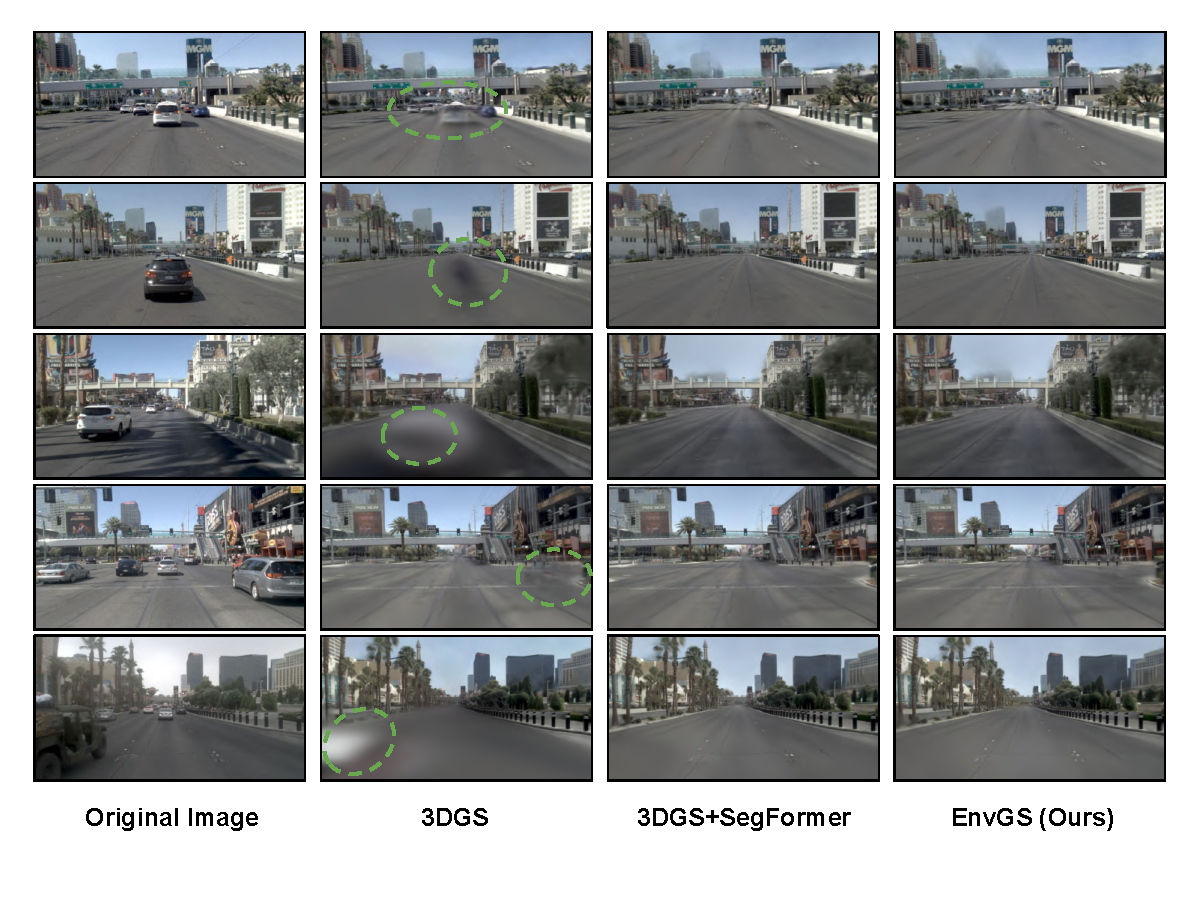
\includegraphics[width=0.925\linewidth]{figs_compressed/nuplan-rendering_compressed.pdf}
    \caption{\textbf{Visualizations of neural rendering in Mapverse-nuPlan.}}
    \label{fig:nuplan-rendering-appendix}
\end{figure}


\clearpage
\section{Limitations and Future Work}
\label{sec:limitation-appendix}

% \emph{(4)} \textit{Future improvements.} Future directions may include the exploration of more powerful foundation models and leveraging the temporal information within each traversal to enhance the consistency of the masks.

\subsection{Unsupervised 2D Segmentation}
\paragraph{Shadow segmentation} Figure~\ref{fig:limitation-shadow-appendix} illustrates the challenges encountered in accurately segmenting shadows. Each row represents different instances. The left column displays the original images, the middle column presents the segmentation output, and the right column highlights the areas where shadow removal failed, indicated by red circles. While there are some successful cases marked by green circles, our method lacks consistency across different scenes. 

\begin{figure}[ht]
    \centering
    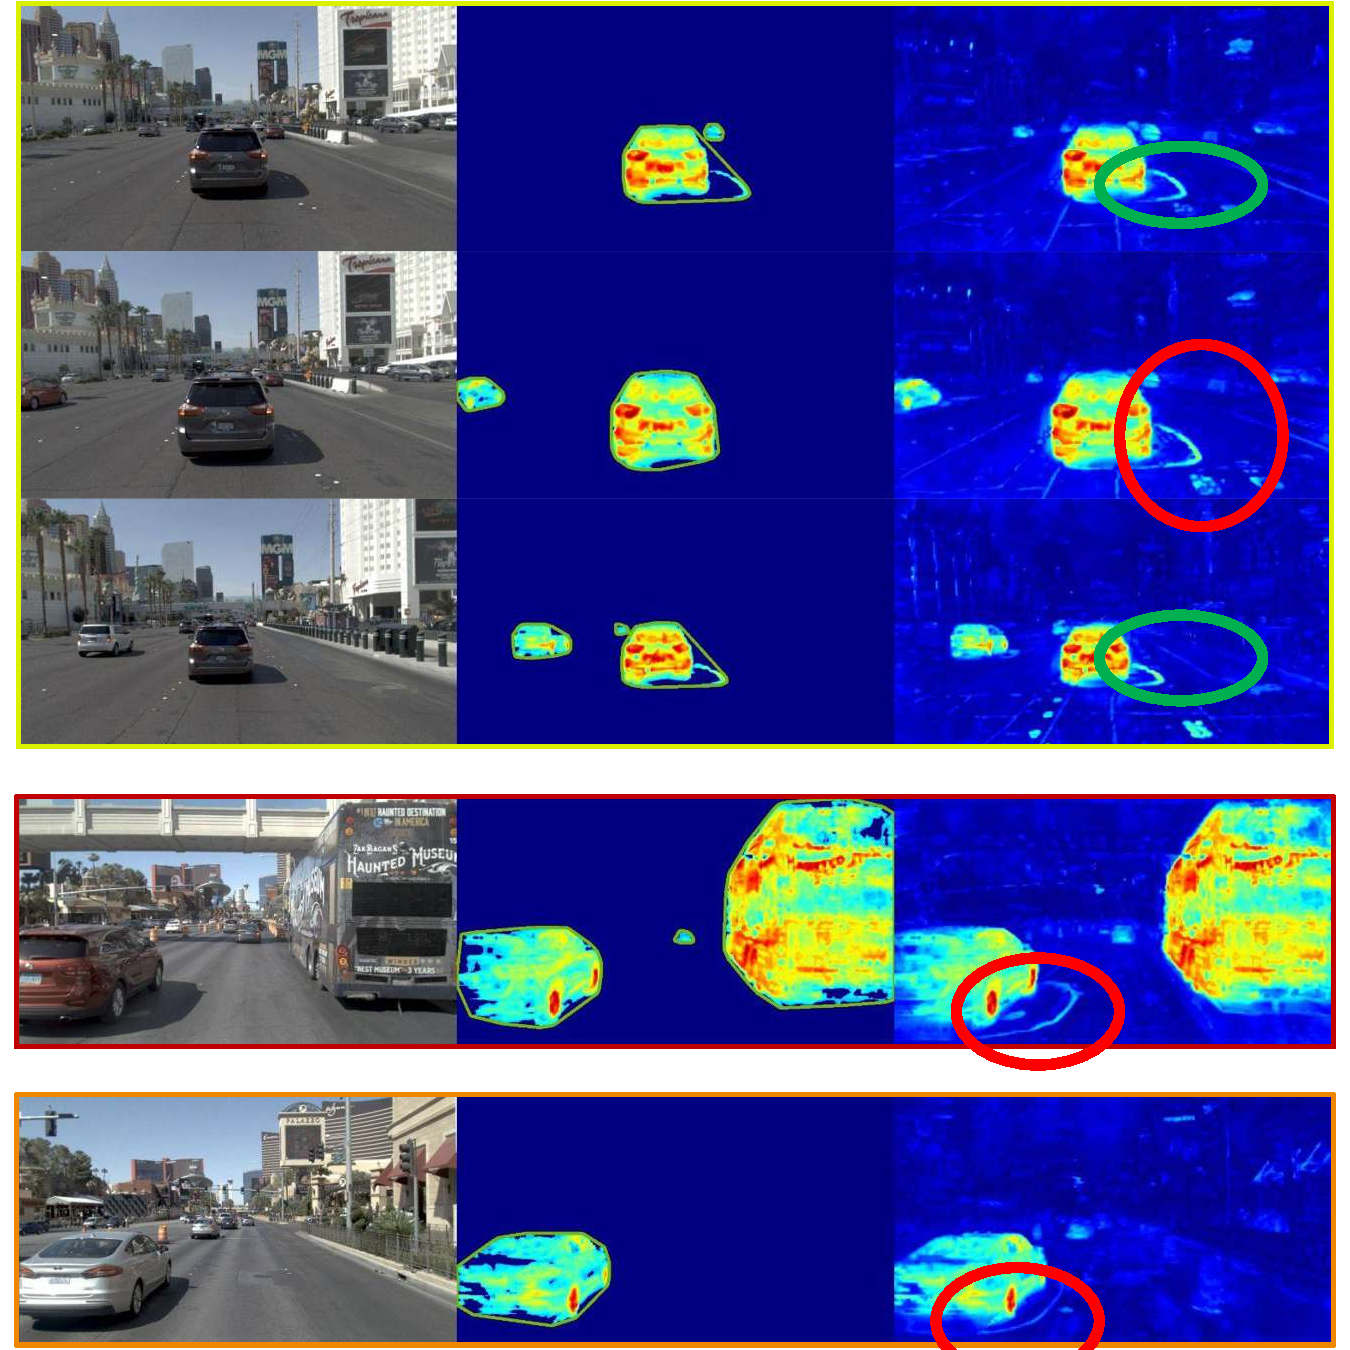
\includegraphics[width=0.66\linewidth]{figs_compressed/limitation-shadow_compressed.pdf}
    \caption{\textbf{Failure cases of shadow segmentation.}}
    \label{fig:limitation-shadow-appendix}
    \vspace{-2mm}
\end{figure}

 \paragraph{Large occluders} Figure~\ref{fig:limitation-large-appendix} illustrates the challenges faced when segmenting scenes with large and enduring occluders. When occluders occupy a significant portion of pixels and persist over time, our model tends to overfit to these occluders. This leads to a reduction in the feature residuals of the corresponding pixels, thereby failing the segmentation.

 \paragraph{Long-range objects} Figure~\ref{fig:limitation-small-appendix} highlights the challenges encountered when segmenting scenes with small and long-range objects. The red circles indicate regions where the segmentation algorithm struggles to differentiate these objects from their surroundings, often missing or inaccurately segmenting them. 

\paragraph{Reflective Surfaces} Figure~\ref{fig:limitation-reflect-appendix}  highlights the model's current limitations in handling reflective surfaces, which can vary significantly across traversals due to changes in lighting.
 
 \paragraph{Future Work} Future work will focus on developing better methods to robustly segment object shadows and leveraging temporal information to more effectively handle large and enduring occluders. Additionally, designing adaptive thresholds based on object distance will help better exploit the spatial information of the feature residuals. Furthermore, training a vision foundation model using large-scale, in-the-wild data will be crucial for enhancing the model's robustness.

\subsection{Geometry Reconstruction}

There are still challenges in road reconstruction, particularly due to the textureless nature of road surfaces. To address this, integrating advanced techniques such as mesh reconstruction~\cite{guedon2023sugar} and 2D Gaussian Splatting~\cite{Huang2DGS2024} could significantly enhance the geometric reconstruction capabilities of our method.  By enhancing the geometric fidelity of road surfaces, these techniques can help overcome the limitations posed by textureless areas, ensuring a more comprehensive and reliable mapping of driving environments.

\subsection{Neural Rendering}
Our method currently struggles with handling significant lighting variations and seasonal changes in the environment. Incorporating a 4D representation~\cite{yang2023gs4d,yan2024street}, which accounts for changes over time, could further enhance the quality of neural rendering. Additionally, we have not yet investigated very large-scale scene reconstruction. Incorporating recent Level-of-Detail (LOD) techniques can help address this large-scale problem~\cite{hierarchicalgaussians24}. We leave these as future works.

 \begin{figure}[ht]
    \centering
    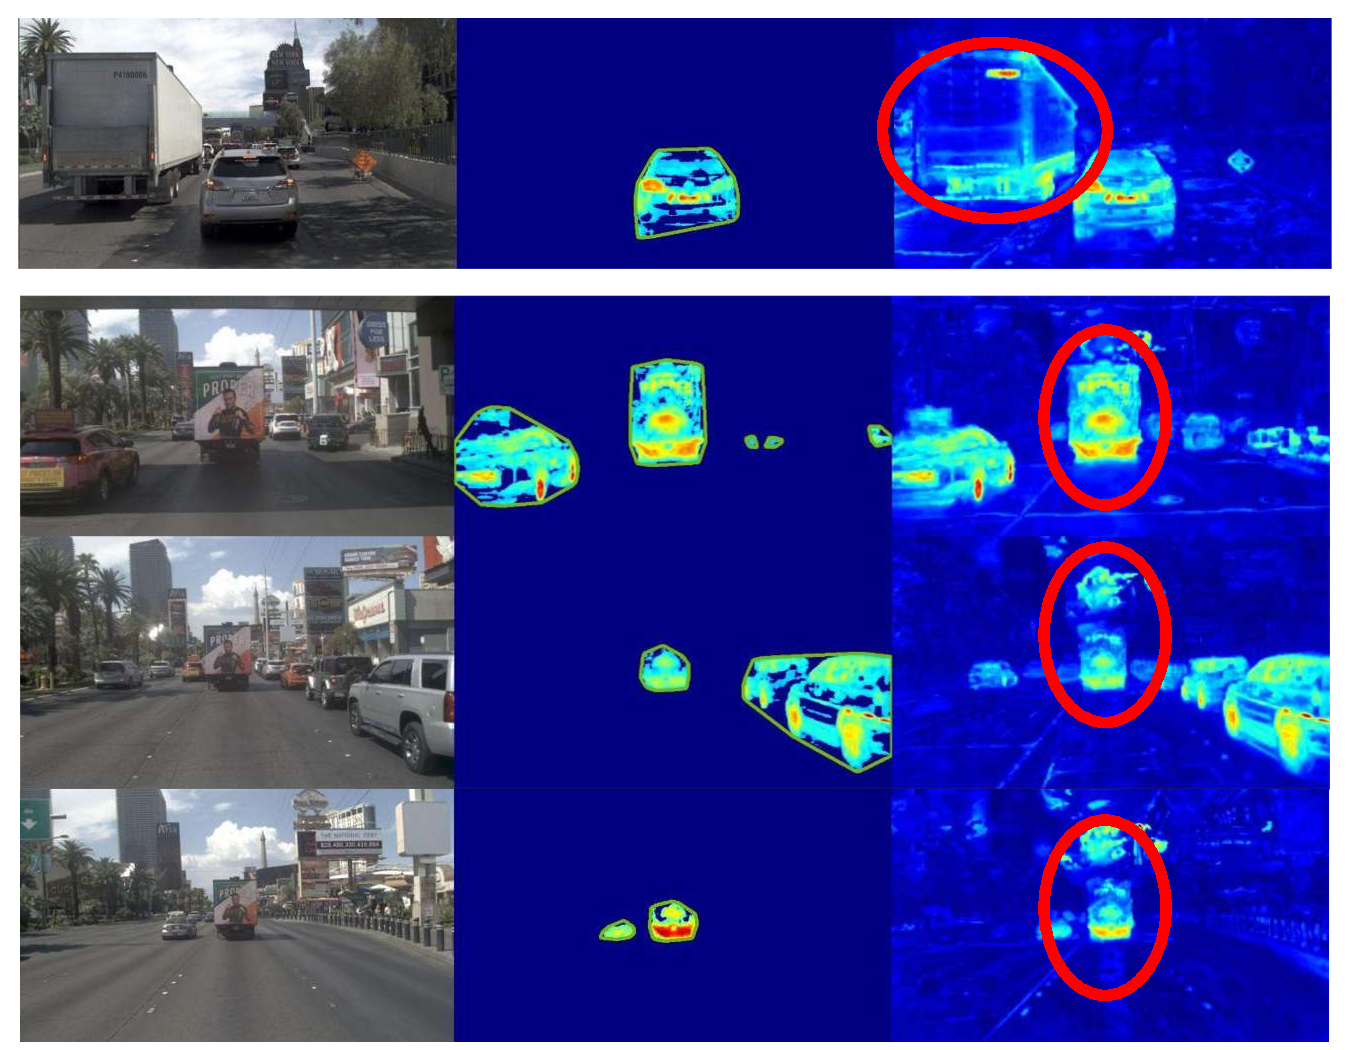
\includegraphics[width=0.66\linewidth]{figs_compressed/limitation-large_compressed.pdf}
    \caption{\textbf{Failure cases when faced with large and enduring occluders.}}
    \label{fig:limitation-large-appendix}
\end{figure}
\begin{figure}[ht]
    \centering
    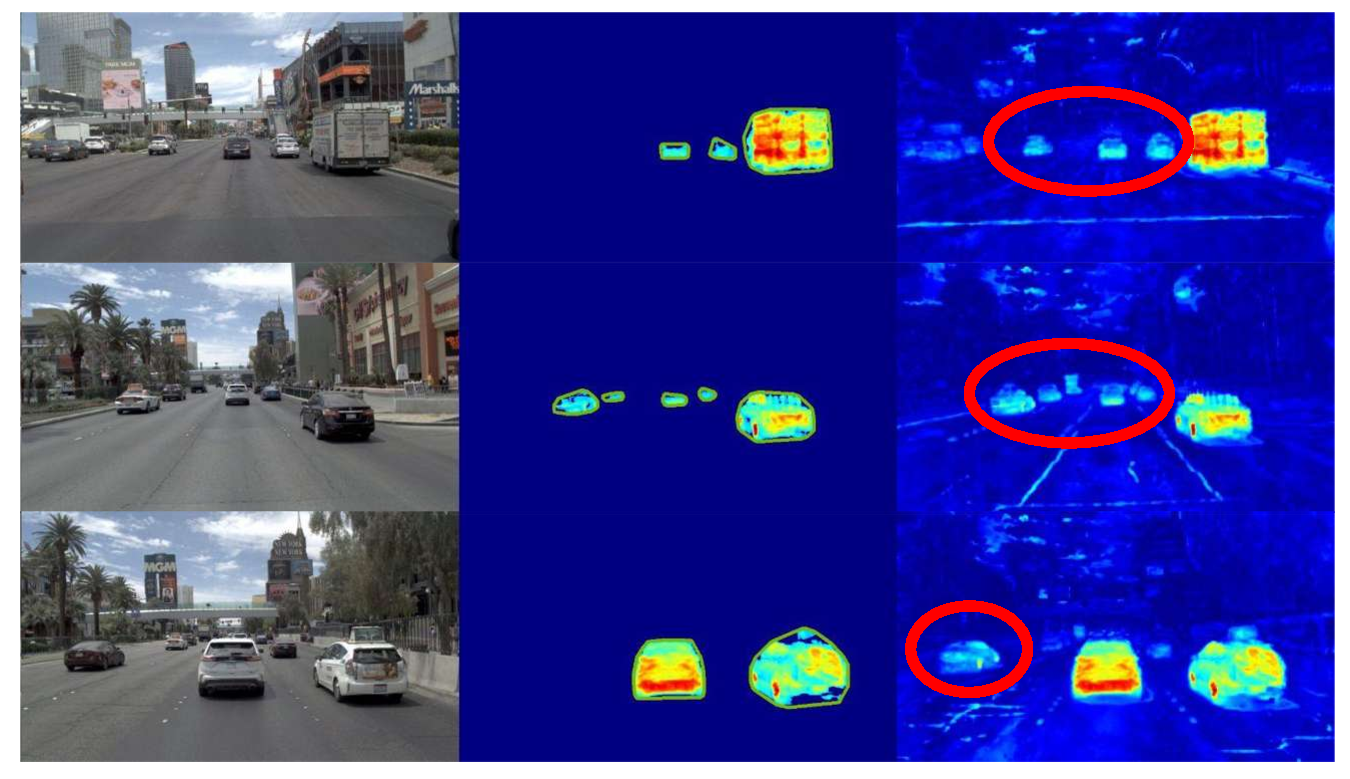
\includegraphics[width=0.66\linewidth]{figs_compressed/limitation-small_compressed.pdf}
    \caption{\textbf{Failure cases when faced with small and long-range objects.}}
    \label{fig:limitation-small-appendix}
\end{figure}
\begin{figure}[ht]
    \centering
    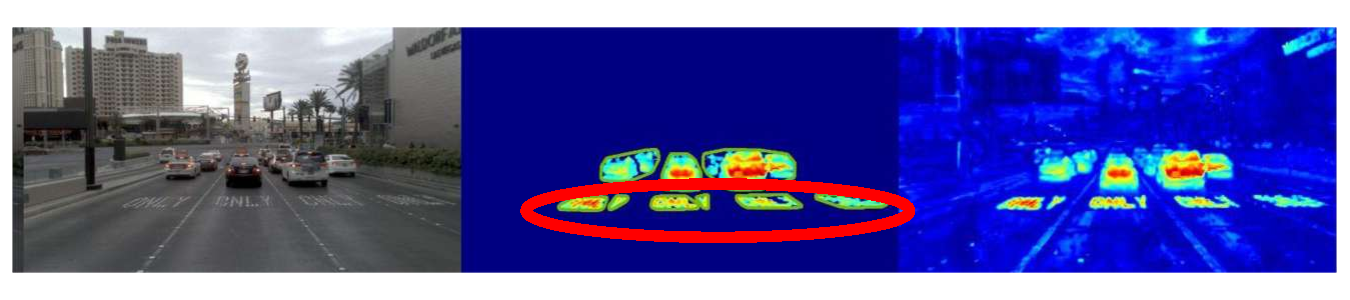
\includegraphics[width=0.66\linewidth]{figs_compressed/limitation-reflect_compressed.pdf}
    \caption{\textbf{Failure cases when faced with reflective surfaces.}}
    \label{fig:limitation-reflect-appendix}
\end{figure}